\documentclass[10pt,dvipsnames]{beamer}
\usepackage[T1]{fontenc}
\usepackage{libertinus}
\usepackage{amsmath}
\usepackage[most]{tcolorbox}
\usepackage{graphicx}

\usepackage{hyperref}
%python 
\usepackage{listings}
% Default fixed font does not support bold face
\DeclareFixedFont{\ttb}{T1}{txtt}{bx}{n}{8} % for bold
\DeclareFixedFont{\ttm}{T1}{txtt}{m}{n}{8}  % for normal

% Custom colors
\usepackage{color}
\definecolor{deepblue}{rgb}{0,0,0.5}
\definecolor{deepred}{rgb}{0.6,0,0}
\definecolor{deepgreen}{rgb}{0,0.5,0}

\usepackage{listings}

% Python style for highlighting
\newcommand\pythonstyle{\lstset{
		language=Python,
		basicstyle=\ttm,
		morekeywords={self},              % Add keywords here
		keywordstyle=\ttb\color{deepblue},
		emph={MyClass,__init__},          % Custom highlighting
		emphstyle=\ttb\color{deepred},    % Custom highlighting style
		stringstyle=\color{deepgreen},
		frame=tb,                         % Any extra options here
		showstringspaces=false
}}


% Python environment
\lstnewenvironment{python}[1][]
{
	\pythonstyle
	\lstset{#1}
}
{}

% Python for external files
\newcommand\pythonexternal[2][]{{
		\pythonstyle
		\lstinputlisting[#1]{#2}}}

% Python for inline
\newcommand\pythoninline[1]{{\pythonstyle\lstinline!#1!}}

\usepackage{xcolor}  
\newcommand{\cb}[1]{{\color{CadetBlue}#1}}

\usepackage{pgfplots}
\pgfplotsset{compat=newest}
\setlength{\parskip}{0.5em}

\usepackage{setspace}
\setstretch{1.25}  
\usetheme{Singapore}
\setbeamertemplate{navigation symbols}{}


\title{CSE574 Introduction to Machine Learning}
\subtitle{Gaussian Naive Bayes}
\author{Jue Guo}
\institute{University at Buffalo}
\date{\today}

\begin{document}
\begin{frame}
    \titlepage
\end{frame}
\begin{frame}
    \frametitle{Outline}
    \tableofcontents
\end{frame}
\section{Learning Objectives}
\begin{frame}{Learning Objectives}
    \begin{itemize}
        \item Define Bayes' rule and conditional probability
        \item Define naive Bayes classification
        \item List and evaluate the assumptions of naive Bayes
        \item Define Gaussian naive Bayes
    \end{itemize}
\end{frame}

\section{Bayes' Rule}
\begin{frame}{Bayes' Rule}
    \begin{itemize}
        \item  The probability an event occurs may change depending on certain conditions. Ex: Not all emails are equally likely to be spam. An email containing the word "URGENT" is more likely to be spam than an email containing the phrase "Meeting". Conditional probability measures the probability that an event occurs, given another event has also occurred.
        \item  The \textbf{conditional probability} of event \(A\), given event \(B\) has already occurred, is denoted as \(P(A \mid B)\).
              $$
                  P(A \mid B)=\frac{P(A \text { and } B)}{P(B)}
              $$
    \end{itemize}
\end{frame}

\begin{frame}
    \frametitle{Bayes' Rule}
    \begin{itemize}
        \item In some cases, the known conditional probability is not the condition of interest.
              \begin{itemize}
                  \item Ex: From a random sample of spam emails,\(P(\) URGENT \(\mid\) Spam \()=0.05\).
                  \item But the conditional probability \(P(\) Spam \(\mid\) URGENT \()\) is more useful for classifying new emails.
              \end{itemize}
              \textbf{Bayes' rule} gives a formula for finding \(P(A \mid B)\) when \(P(B \mid A)\) is known.
              $$
                  P(A \mid B)=\frac{P(B \mid A) \times P(A)}{P(B)}
              $$
    \end{itemize}
\end{frame}

\begin{frame}{Applying Bayes' rule to the penguins data.}
    \begin{figure}[ht]
        \centering
        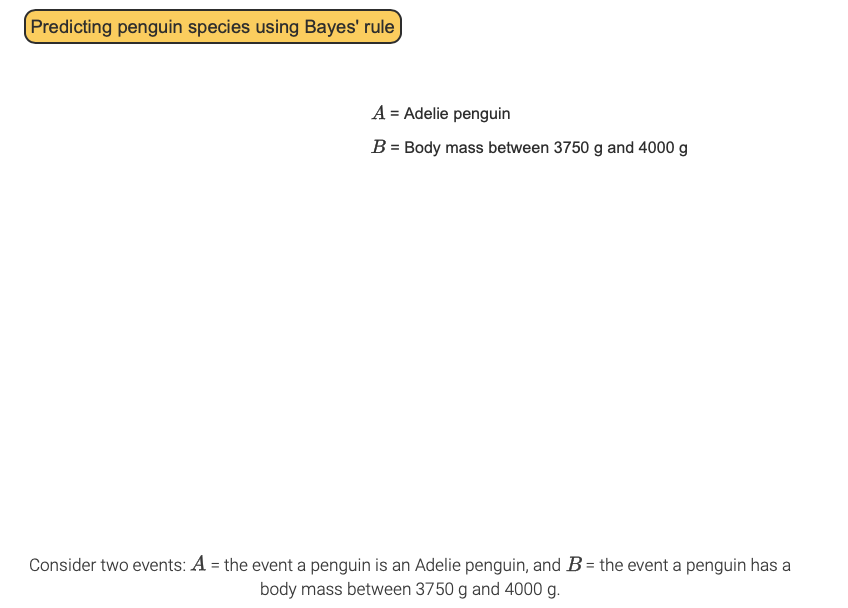
\includegraphics[width=0.8\textwidth]{imgs/nb_1.png}
    \end{figure}
\end{frame}

\begin{frame}{Applying Bayes' rule to the penguins data.}
    \begin{figure}[ht]
        \centering
        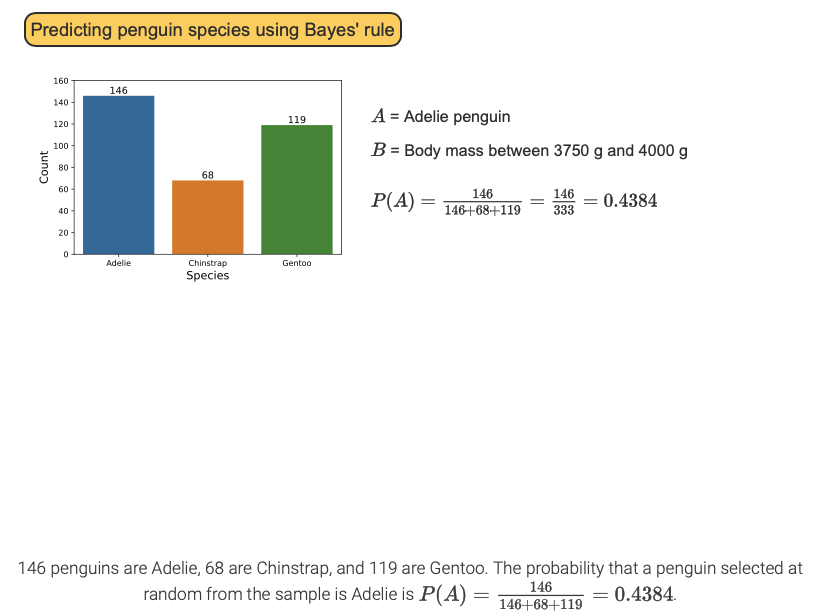
\includegraphics[width=0.8\textwidth]{imgs/nb_2.png}
    \end{figure}
\end{frame}

\begin{frame}{Applying Bayes' rule to the penguins data.}
    \begin{figure}[ht]
        \centering
        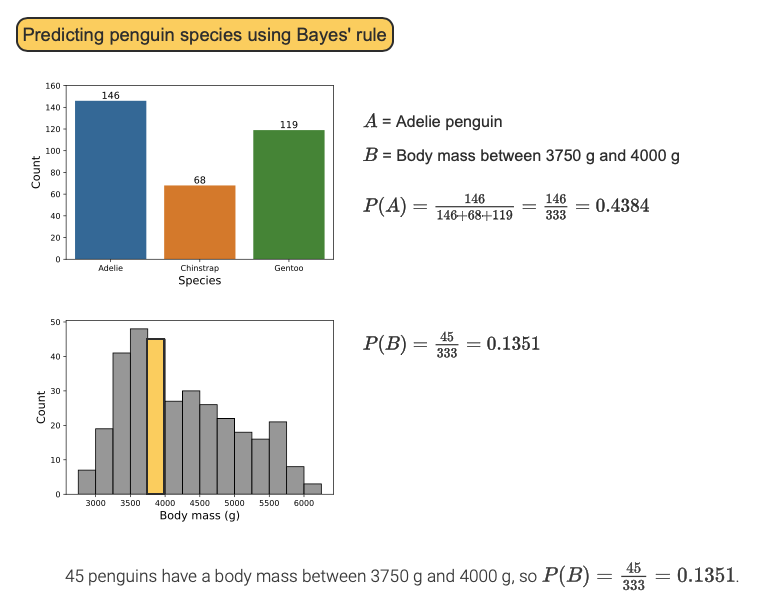
\includegraphics[width=0.8\textwidth]{imgs/nb_3.png}
    \end{figure}
\end{frame}

\begin{frame}{Applying Bayes' rule to the penguins data.}
    \begin{figure}[ht]
        \centering
        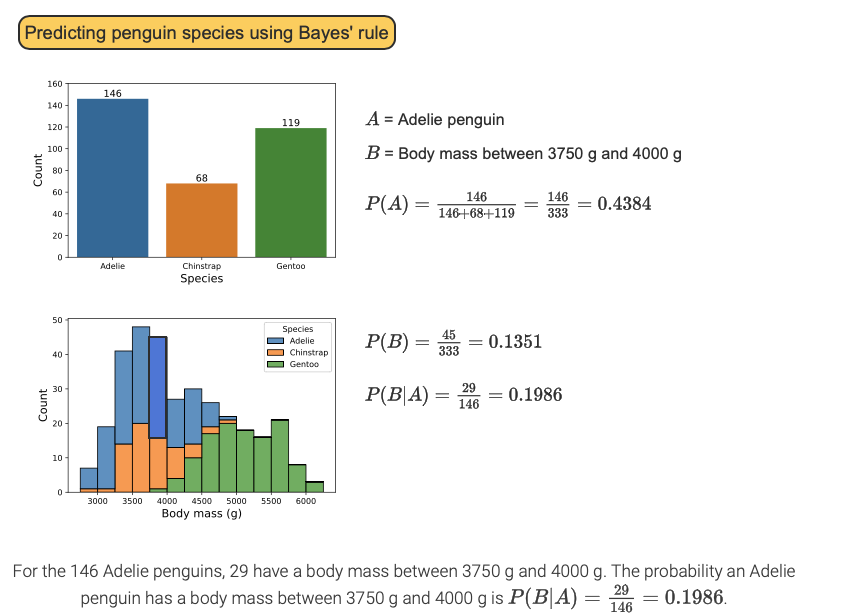
\includegraphics[width=0.8\textwidth]{imgs/nb_4.png}
    \end{figure}
\end{frame}

\begin{frame}{Applying Bayes' rule to the penguins data.}
    \begin{figure}[ht]
        \centering
        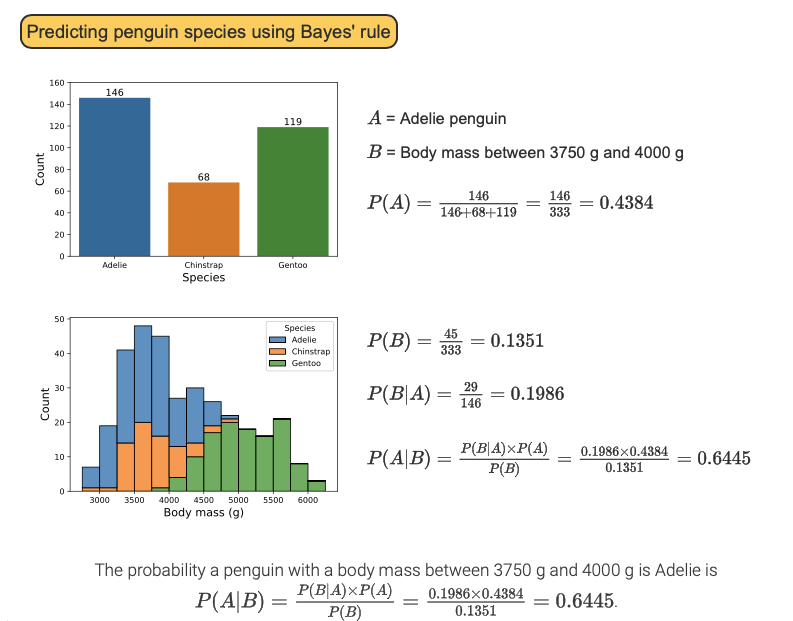
\includegraphics[width=0.8\textwidth]{imgs/nb_5.png}
    \end{figure}
\end{frame}

\begin{frame}{Practice Question: Calculating conditional probabilities}
    \begin{figure}[ht]
        \centering
        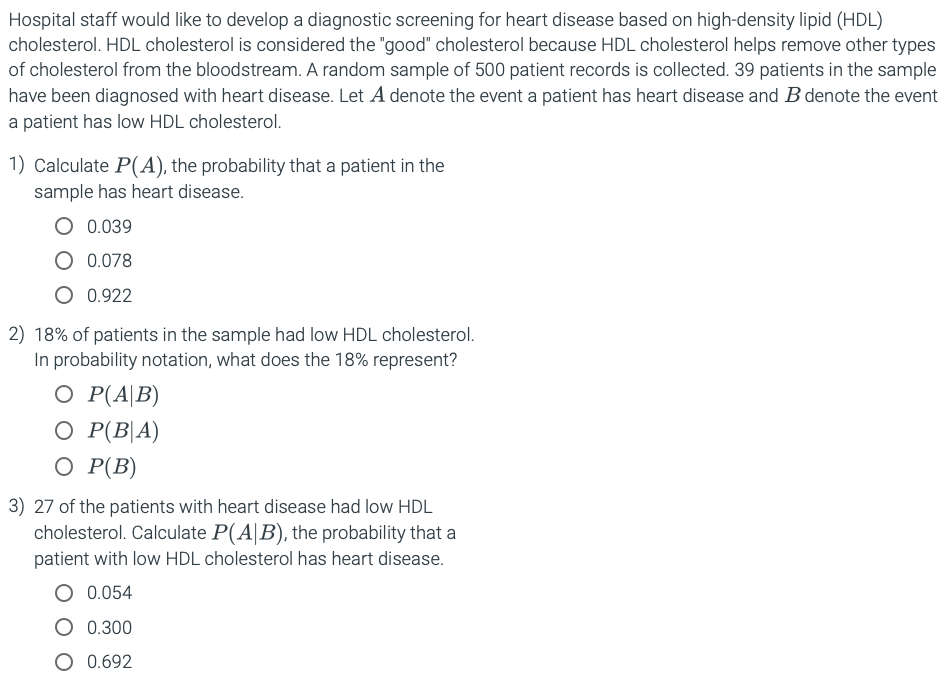
\includegraphics[width=0.8\textwidth]{imgs/nb_6.png}
    \end{figure}
\end{frame}

\begin{frame}{Practice Question: Calculating conditional probabilities}
    \begin{figure}[ht]
        \centering
        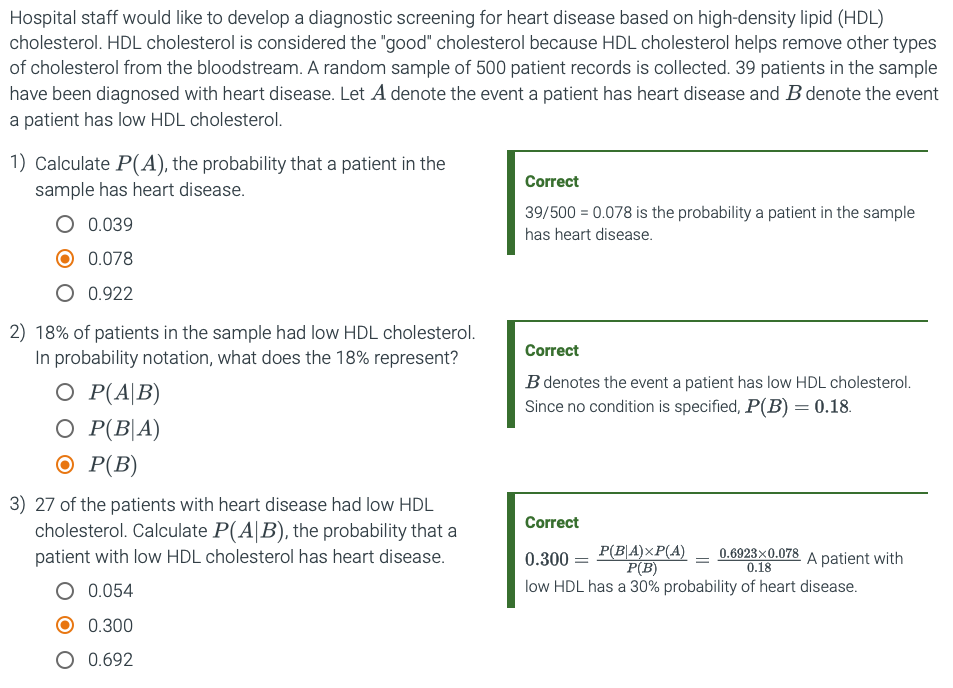
\includegraphics[width=0.8\textwidth]{imgs/nb_7.png}
    \end{figure}
\end{frame}
\section{Naive Bayes Classifier}
\begin{frame}{Naive Bayes Classifier}
	\textbf{Naive Bayes classifier} uses Bayes' rule to classify instances based on conditional probabilities. Let \(y_{i}\) denote class \(i\) of the output feature
	and \(x\) denote the input features. 
	\begin{itemize}
		\item The \textbf{prior probability} represents the overall probability of class \(i\), denoted \(P\left(y_{i}\right)\). 
		
		\item The \textbf{posterior probability} represents the probability of class \(i\), given certain values of the input features \(x\), denoted \(P\left(y_{i} \mid x\right)\) Naive Bayes classifiers make predictions by calculating the posterior probabilities for all \(c\) classes.
	\end{itemize}
	 By Bayes' rule,
	$$
	P\left(y_{i} \mid x\right)=\frac{P\left(x \mid y_{i}\right) \times P\left(y_{i}\right)}{P(x)}
	$$
	The class with the highest posterior probability becomes the predicted class for instance \(i\)
\end{frame}

\begin{frame}{Classifying penguins using naive Bayes.}
	    \begin{figure}[ht]
		\centering
		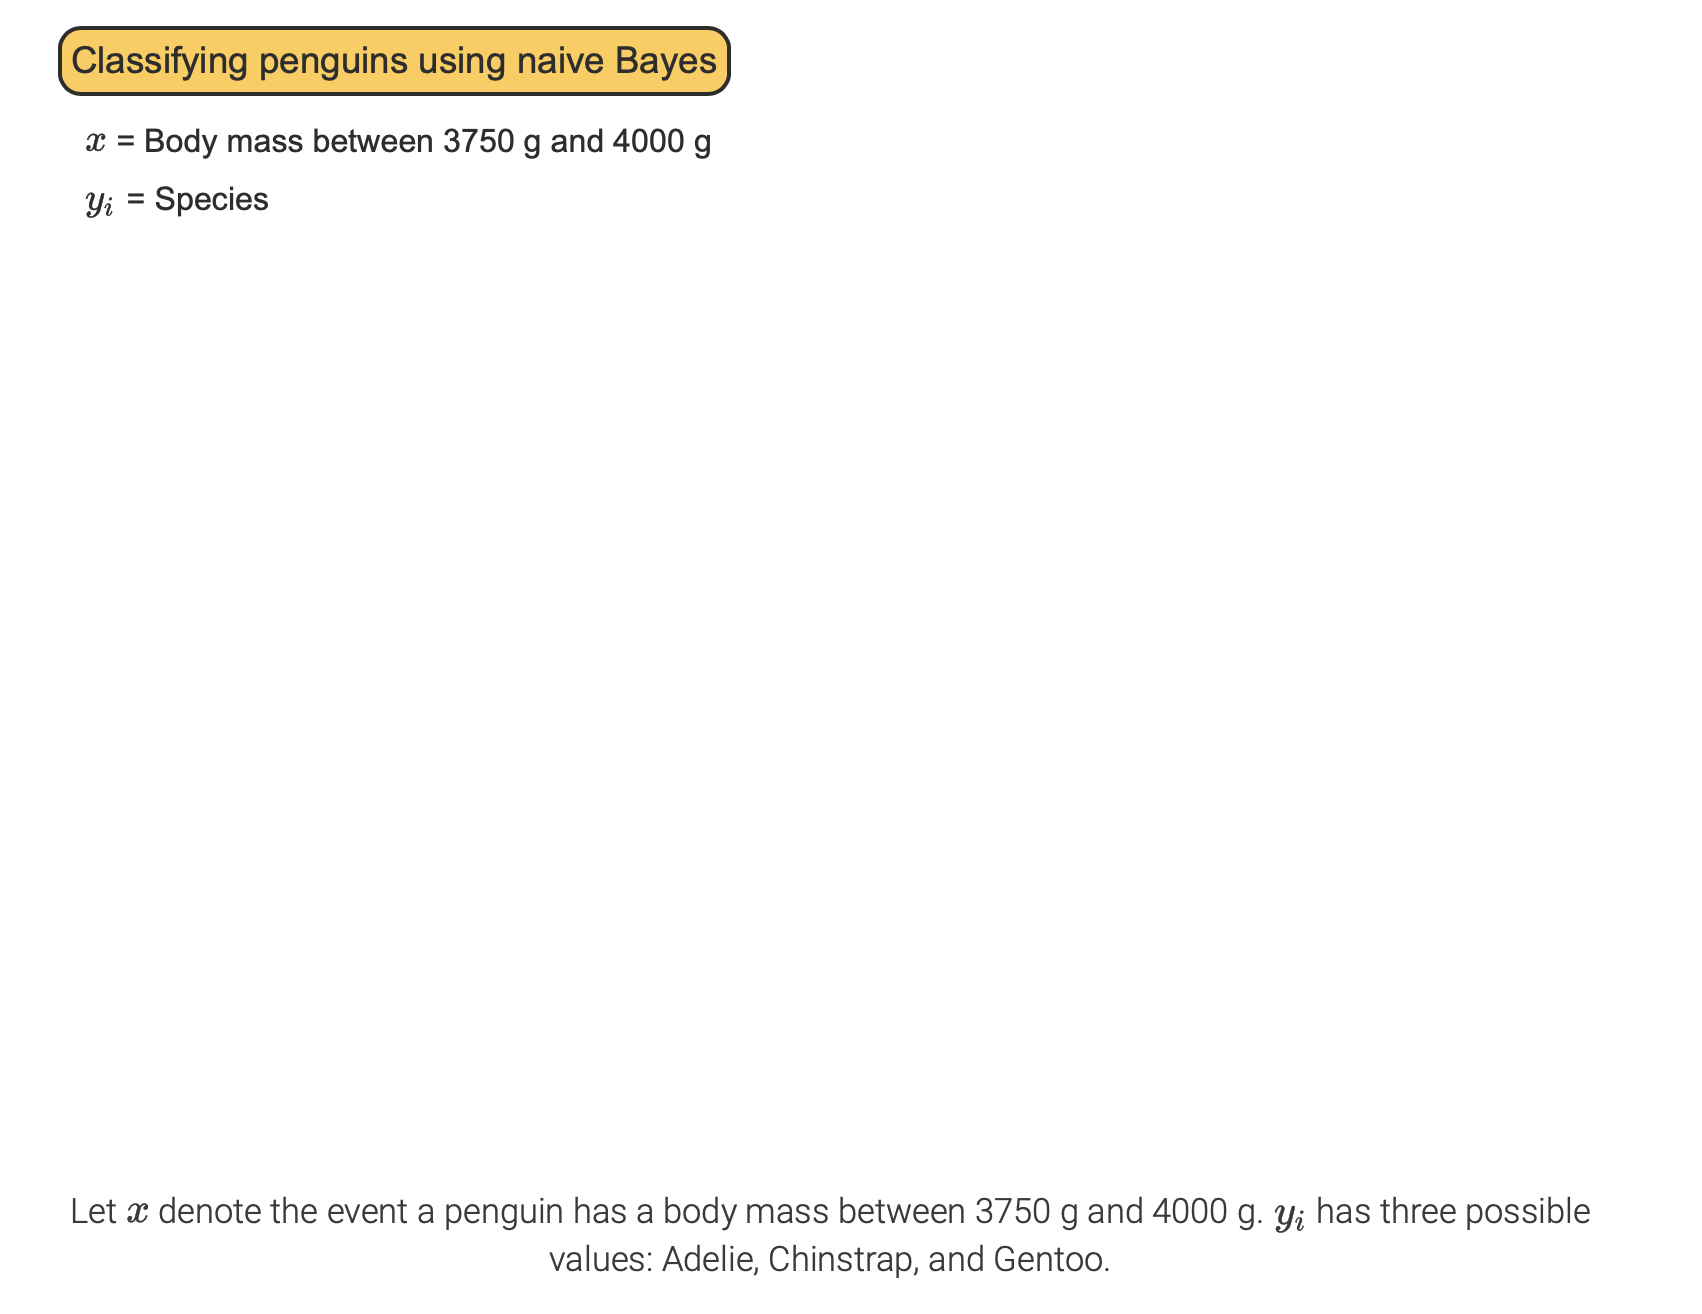
\includegraphics[width=0.8\textwidth]{imgs/nb_8.png}
	\end{figure}
\end{frame}

\begin{frame}{Classifying penguins using naive Bayes.}
	\begin{figure}[ht]
		\centering
		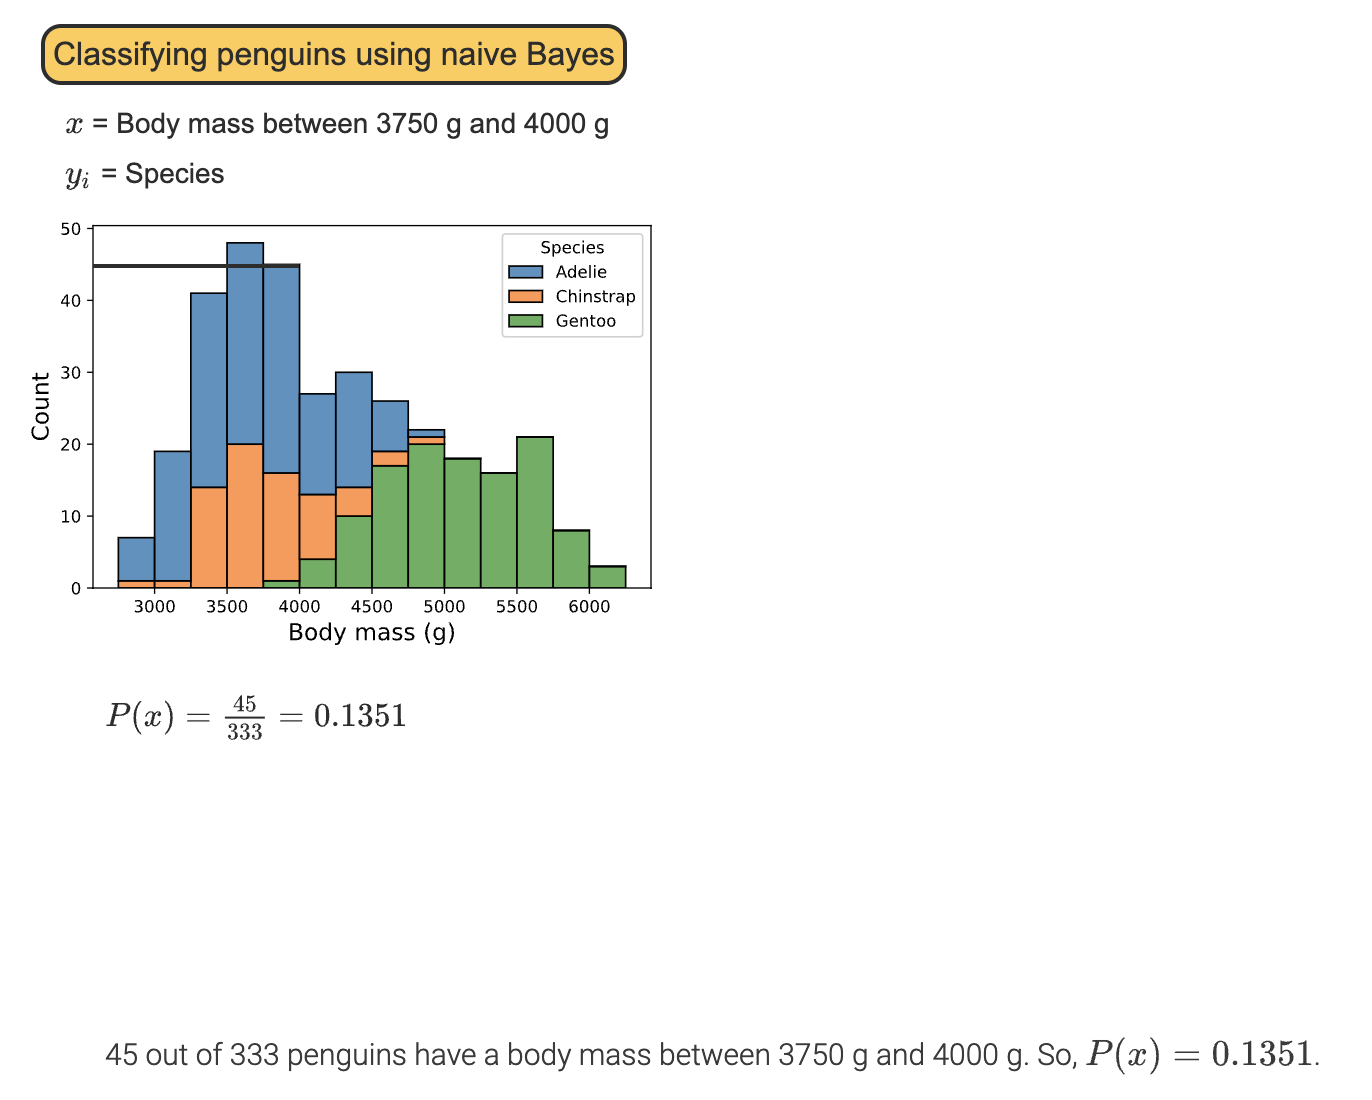
\includegraphics[width=0.8\textwidth]{imgs/nb_9.png}
	\end{figure}
\end{frame}

\begin{frame}{Classifying penguins using naive Bayes.}
	\begin{figure}[ht]
		\centering
		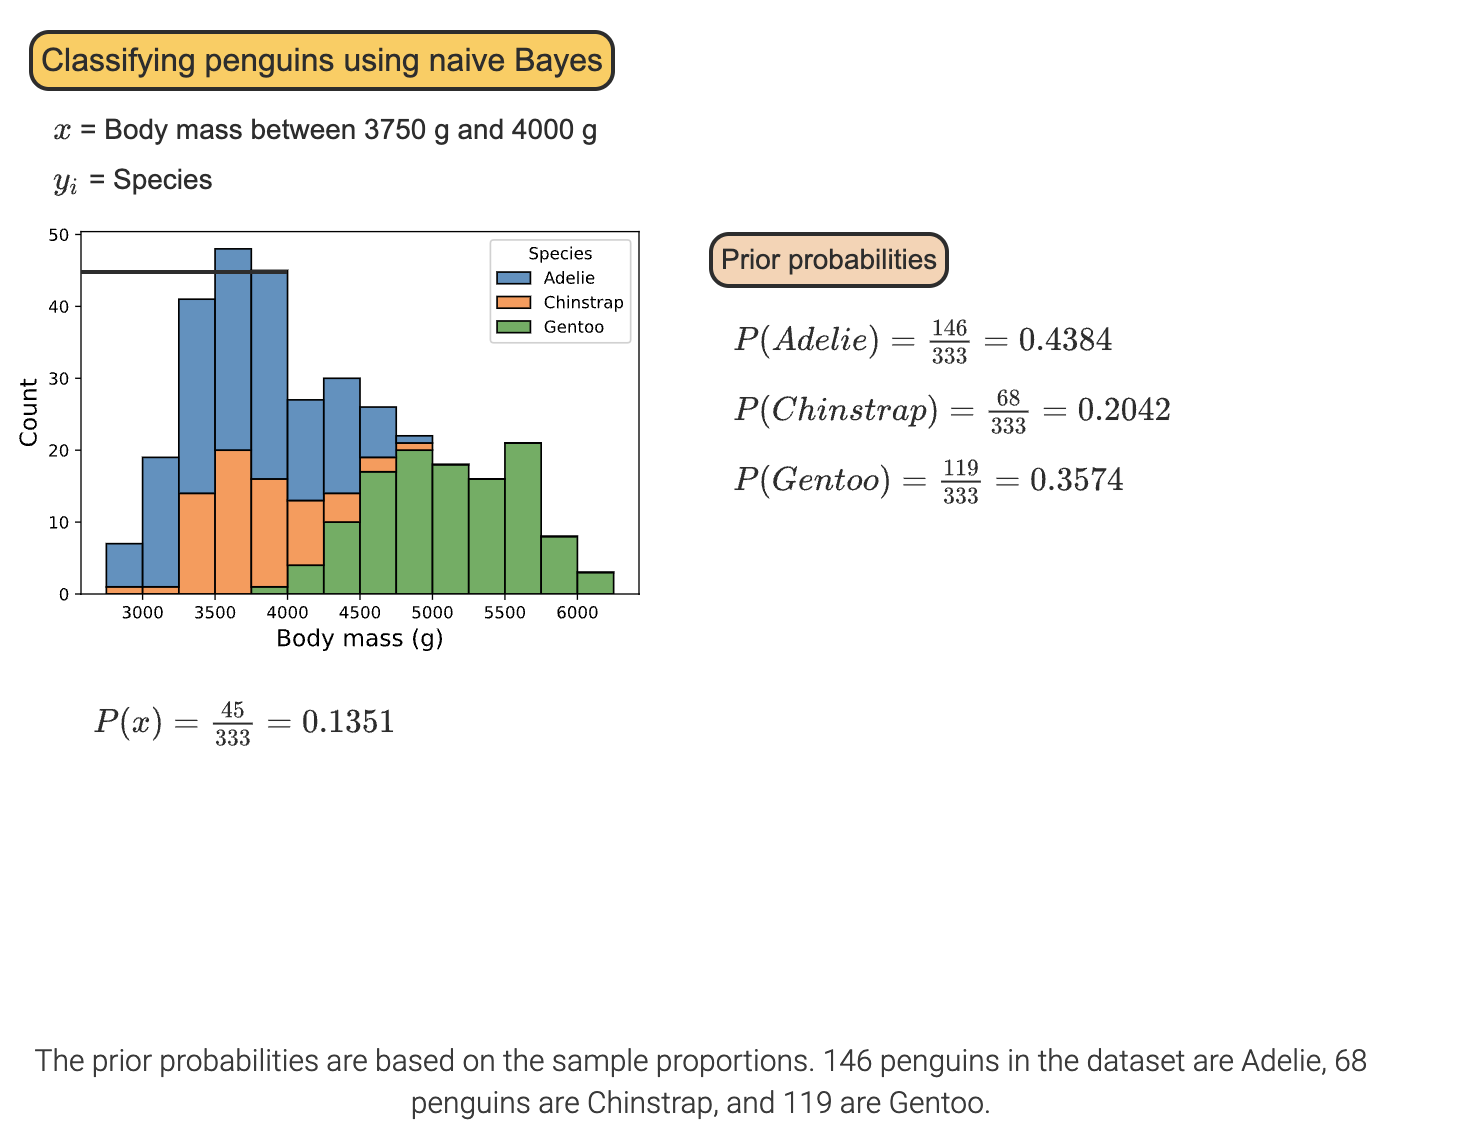
\includegraphics[width=0.8\textwidth]{imgs/nb_10.png}
	\end{figure}
\end{frame}

\begin{frame}{Classifying penguins using naive Bayes.}
	\begin{figure}[ht]
		\centering
		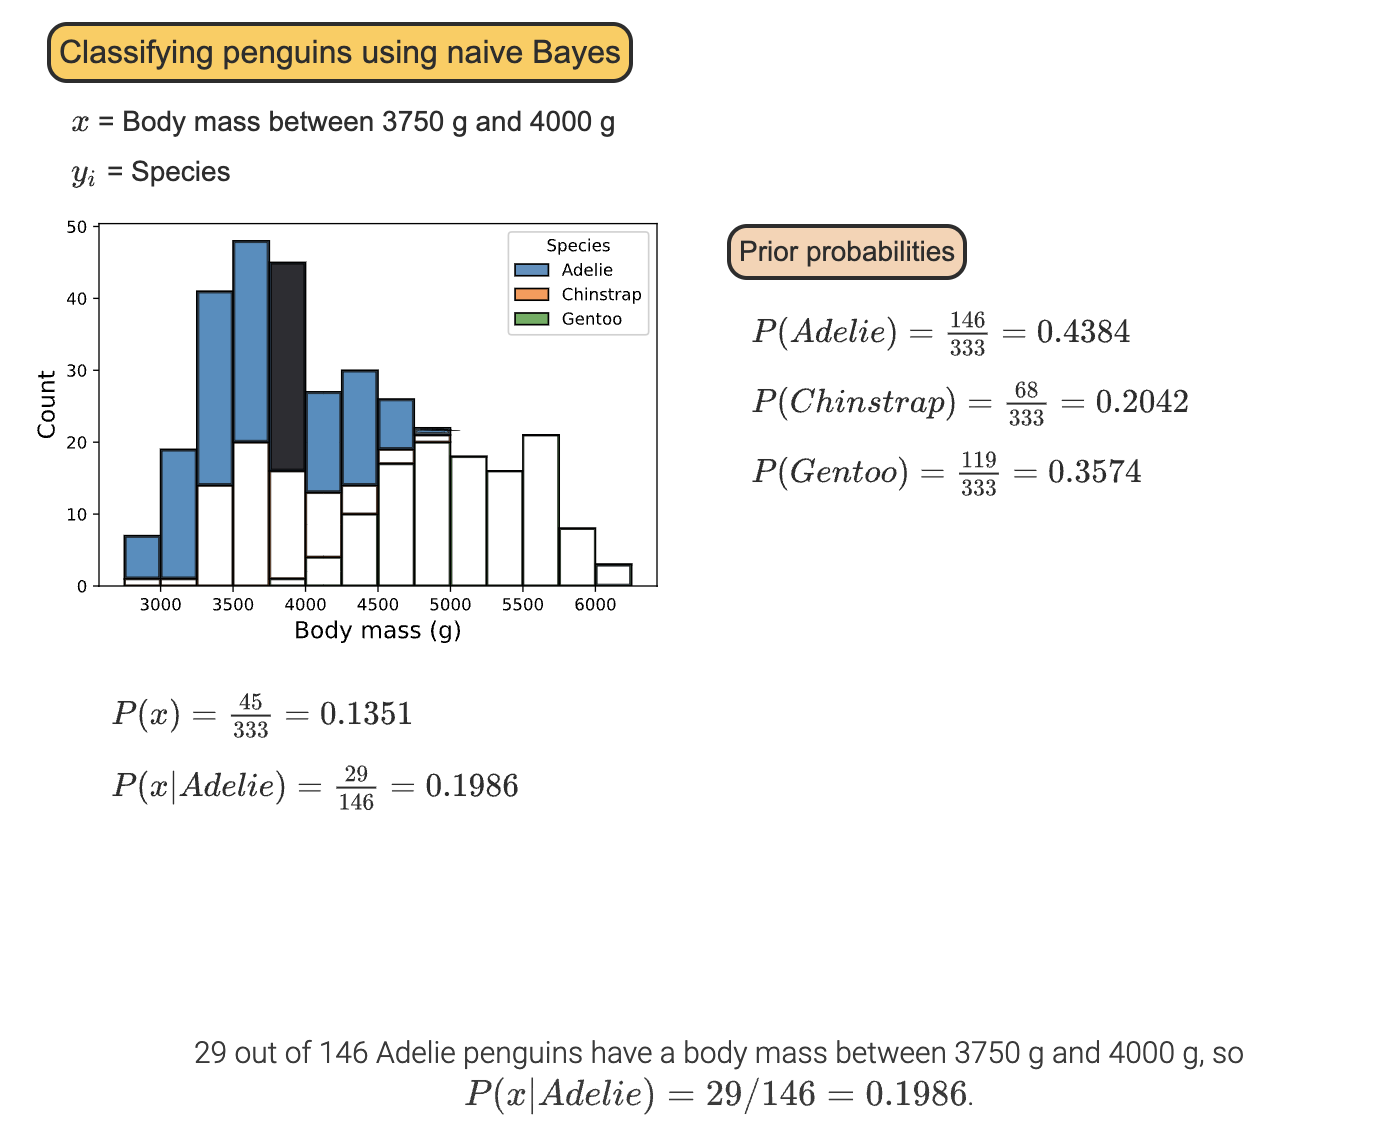
\includegraphics[width=0.8\textwidth]{imgs/nb_11.png}
	\end{figure}
\end{frame}

\begin{frame}{Classifying penguins using naive Bayes.}
	\begin{figure}[ht]
		\centering
		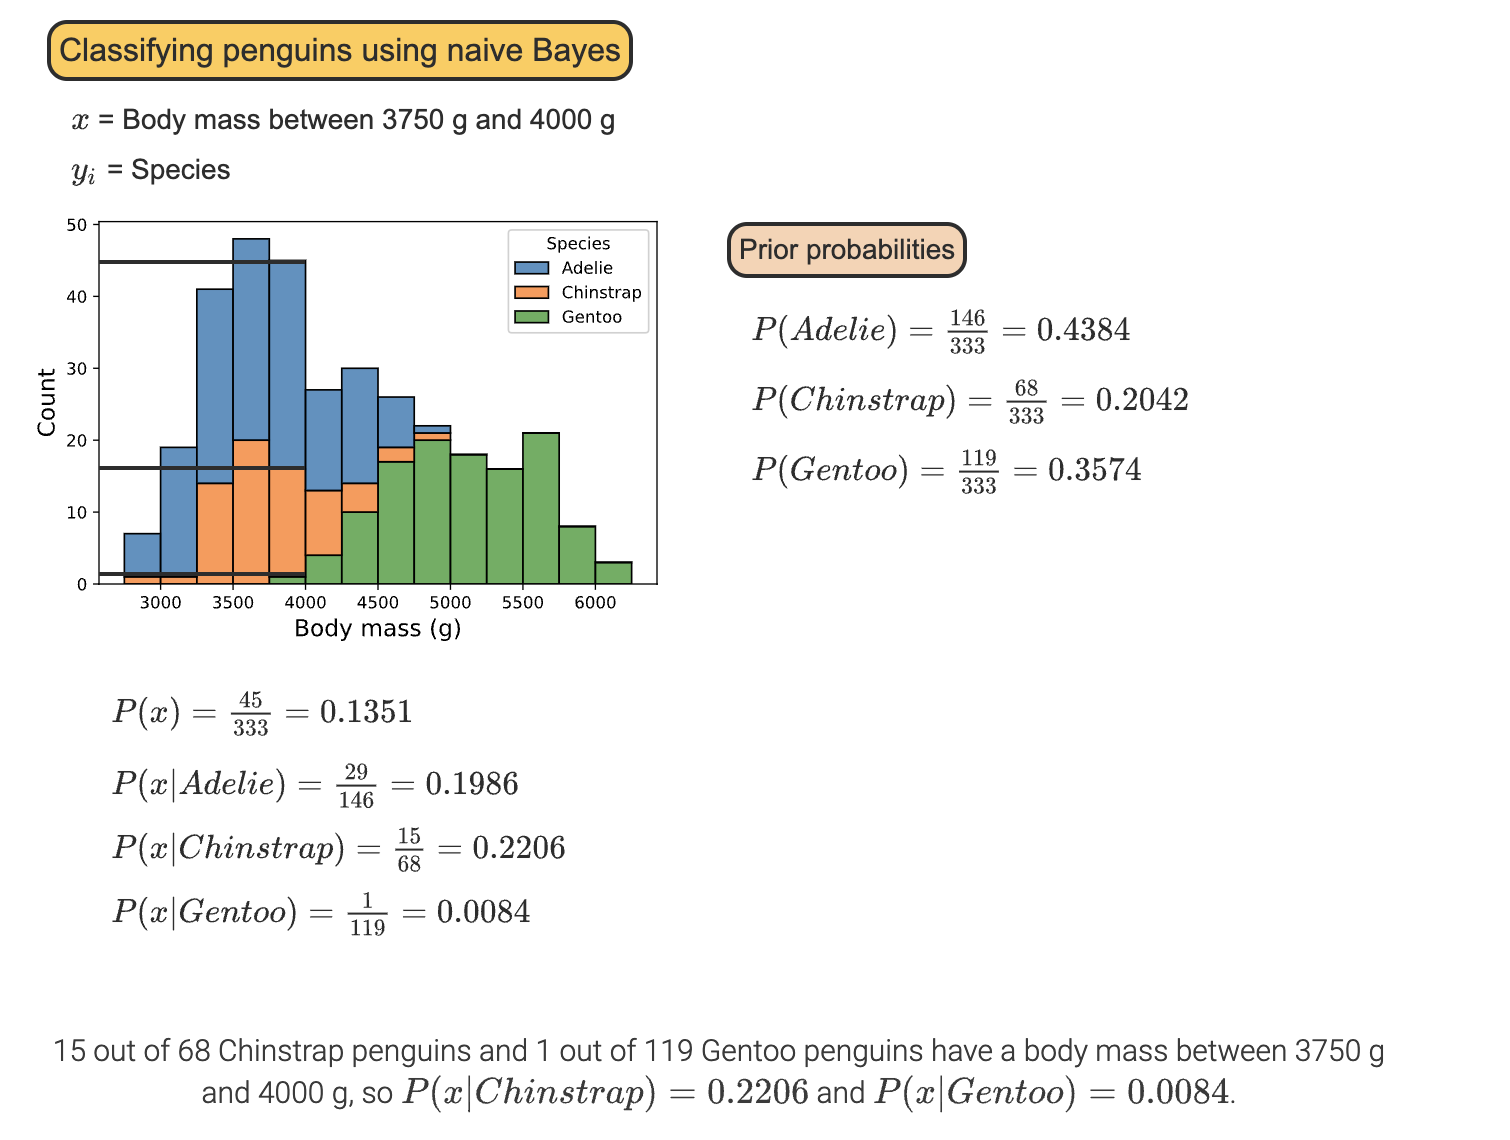
\includegraphics[width=0.8\textwidth]{imgs/nb_12.png}
	\end{figure}
\end{frame}

\begin{frame}{Classifying penguins using naive Bayes.}
	\begin{figure}[ht]
		\centering
		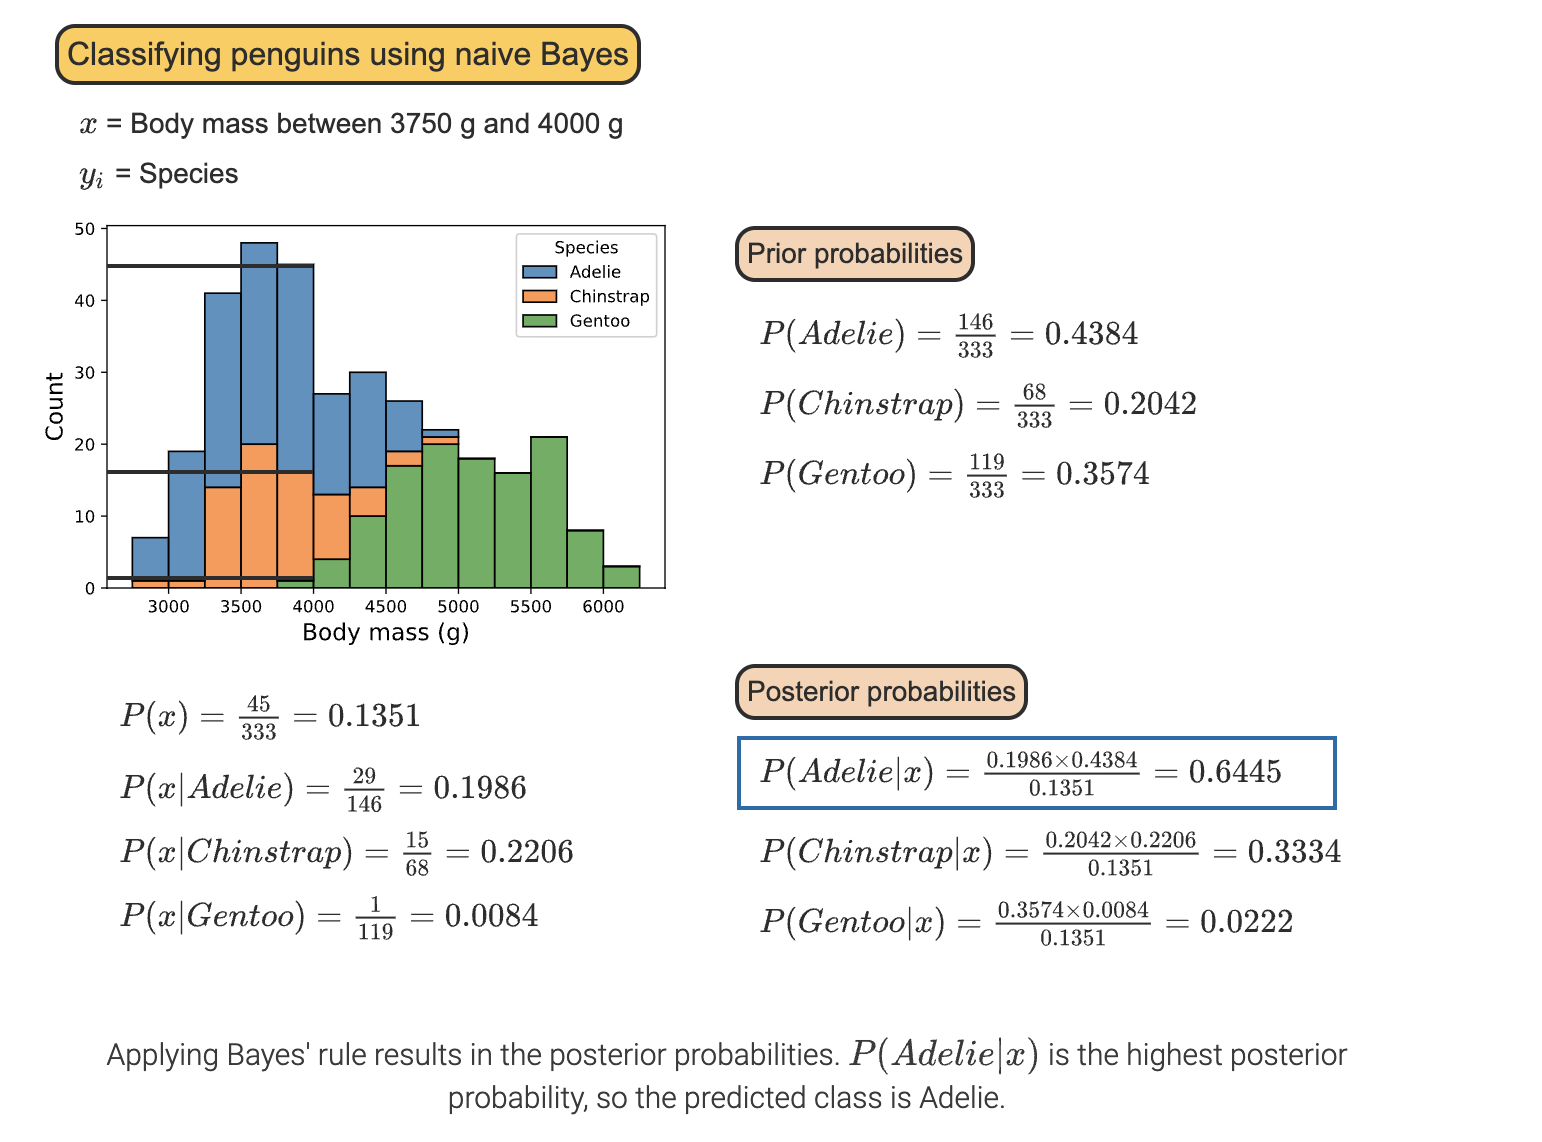
\includegraphics[width=0.8\textwidth]{imgs/nb_13.png}
	\end{figure}
\end{frame}

\begin{frame}{Classifying penguins using naive Bayes.}
	\begin{figure}[ht]
		\centering
		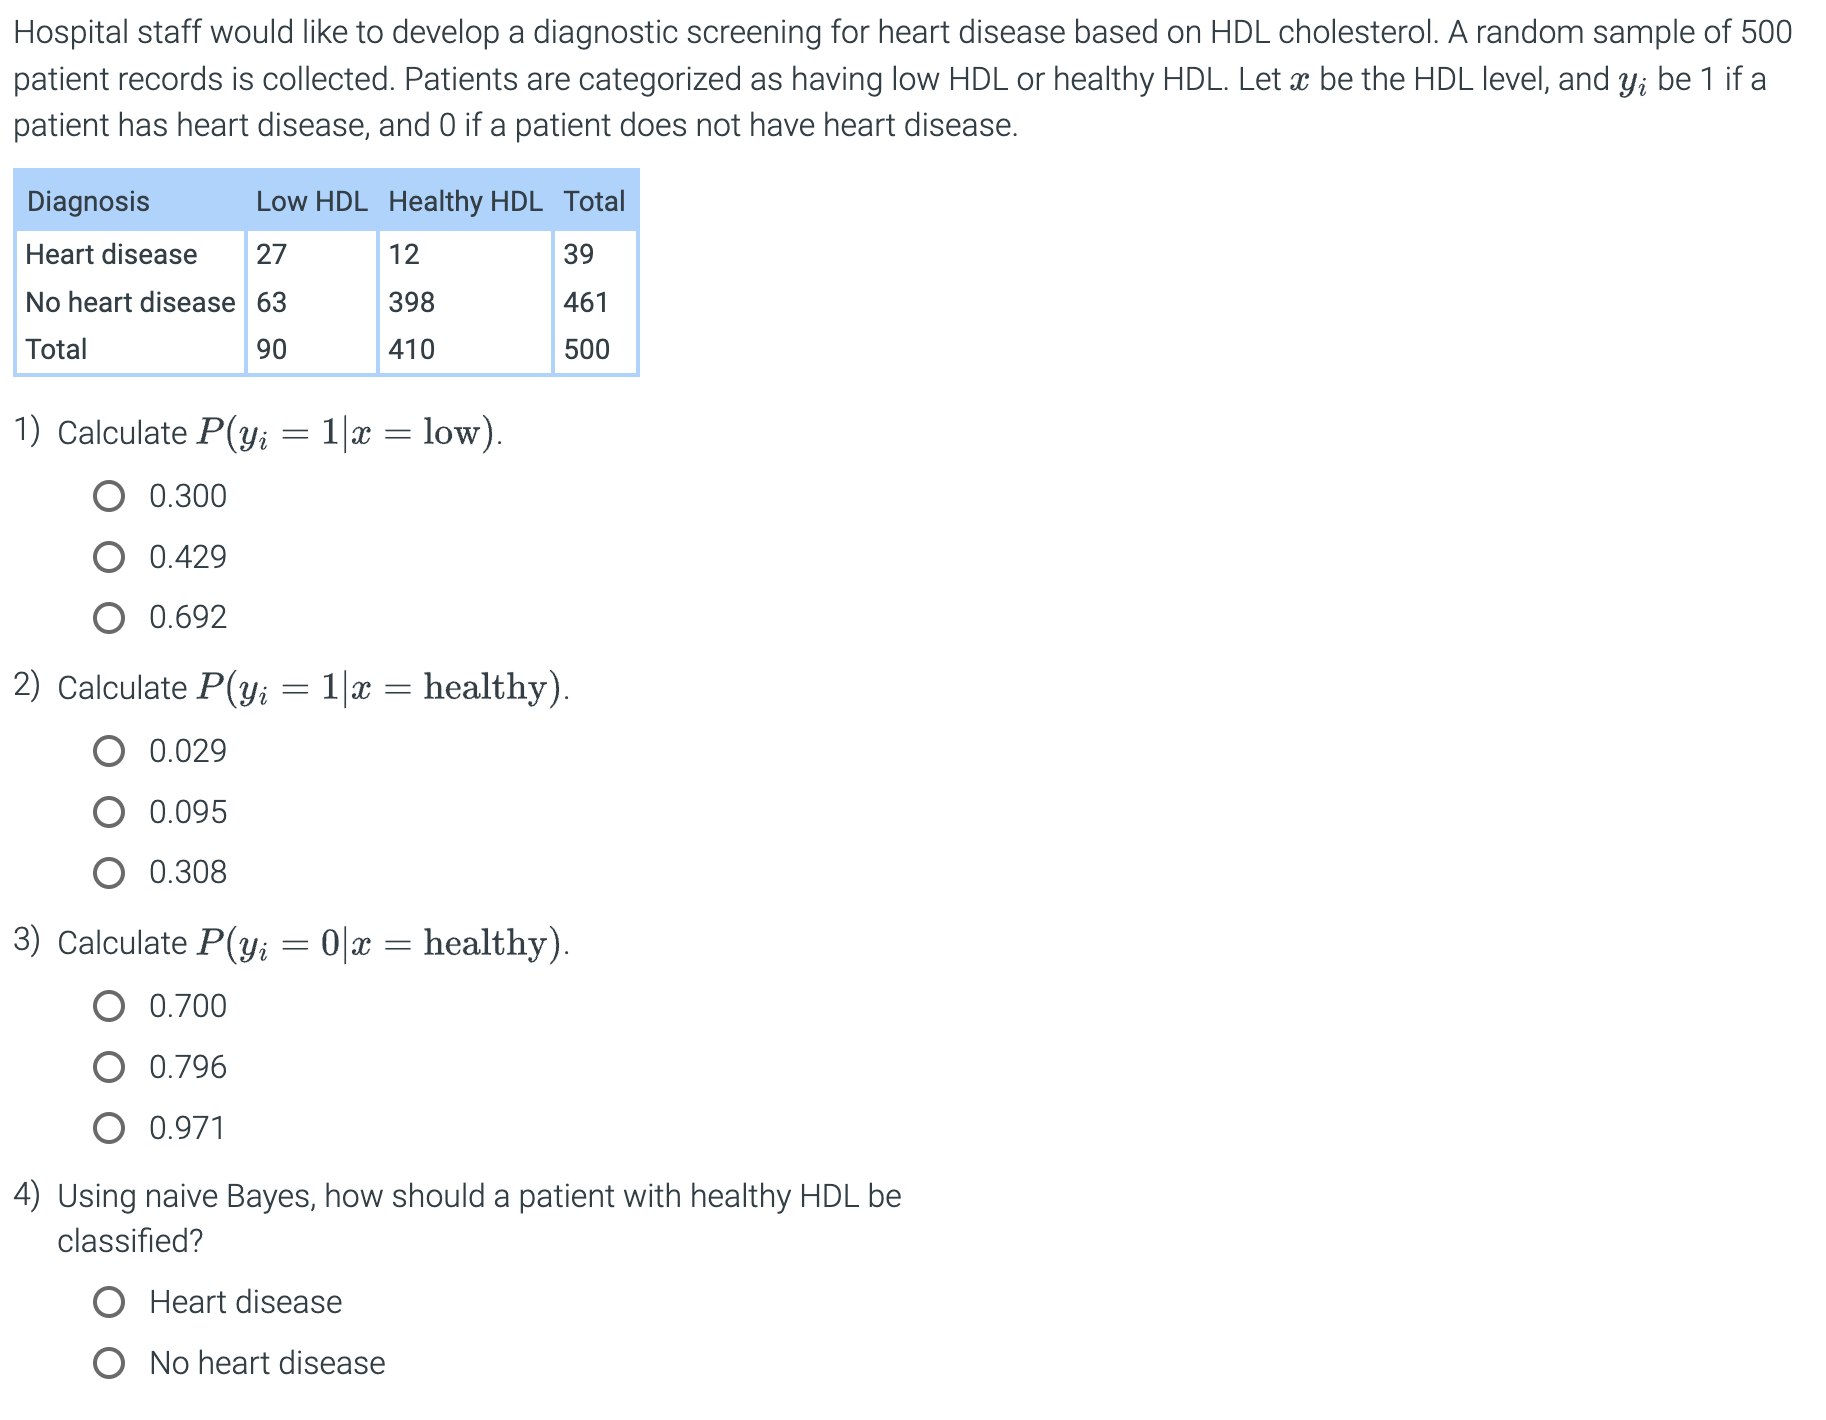
\includegraphics[width=0.8\textwidth]{imgs/nb_14.png}
	\end{figure}
\end{frame}

\begin{frame}{Classifying penguins using naive Bayes.}
	\begin{figure}[ht]
		\centering
		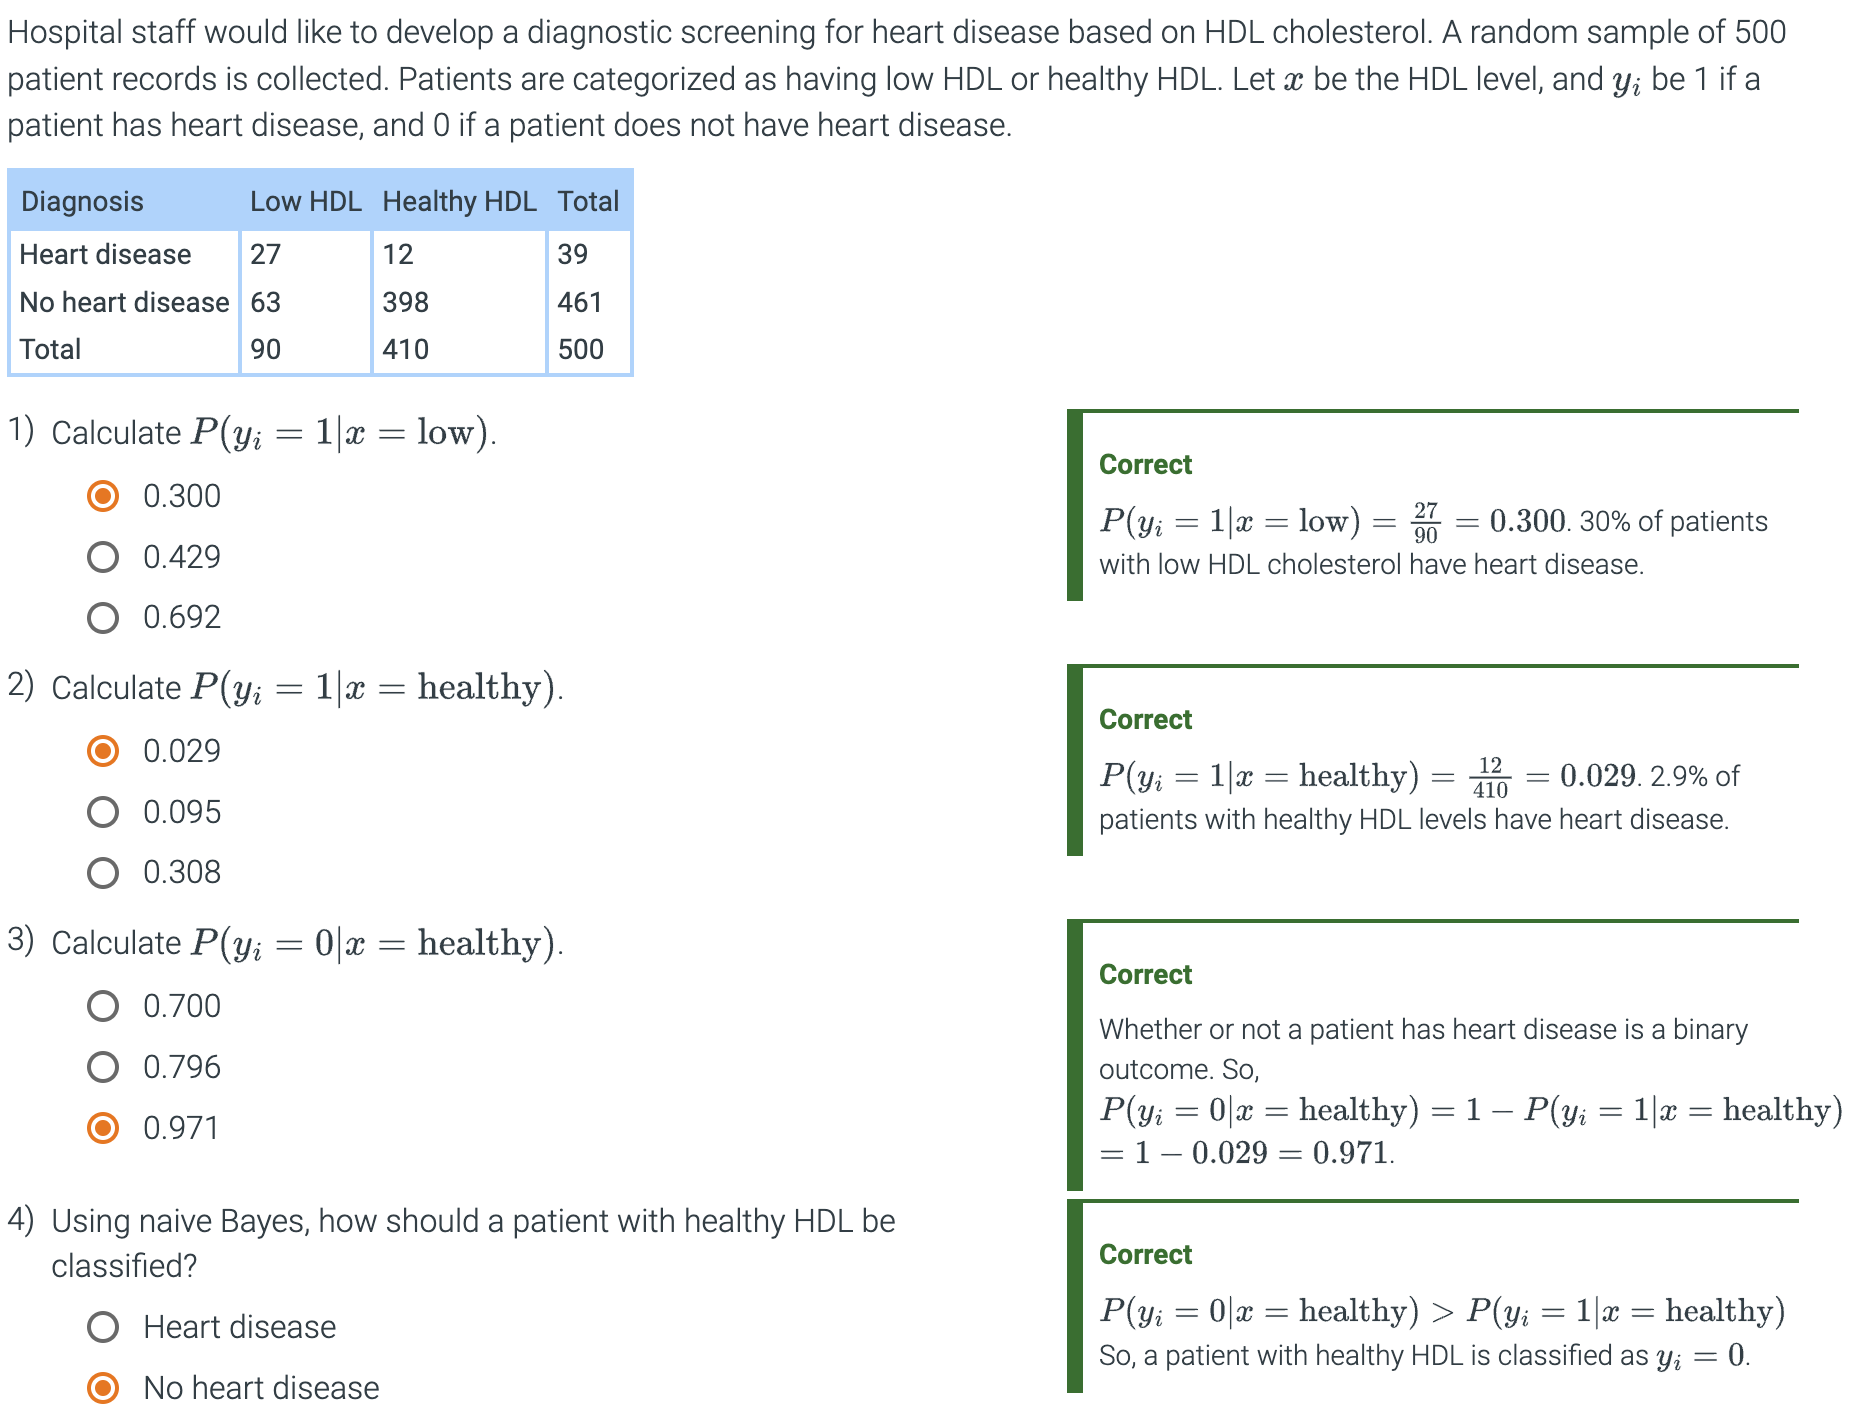
\includegraphics[width=0.8\textwidth]{imgs/nb_15.png}
	\end{figure}
\end{frame}

\section{Naive Bayes Assumptions}
\begin{frame}{Naive Bayes Assumptions}
The name ``naive Bayes" refers to a set of assumptions built into the naive Bayes classifier. Naive Bayes classification assumes:
\begin{enumerate}
	\item All input features are independent or uncorrelated.
	\item All input features are equally important.
\end{enumerate}
But in reality, the naive Bayes assumptions are rarely satisfied. The naive Bayes assumptions can be evaluated by exploring the input features and the data context.
\end{frame}

\begin{frame}{Naive Bayes Assumptions}
	\begin{figure}[ht]
		\centering
		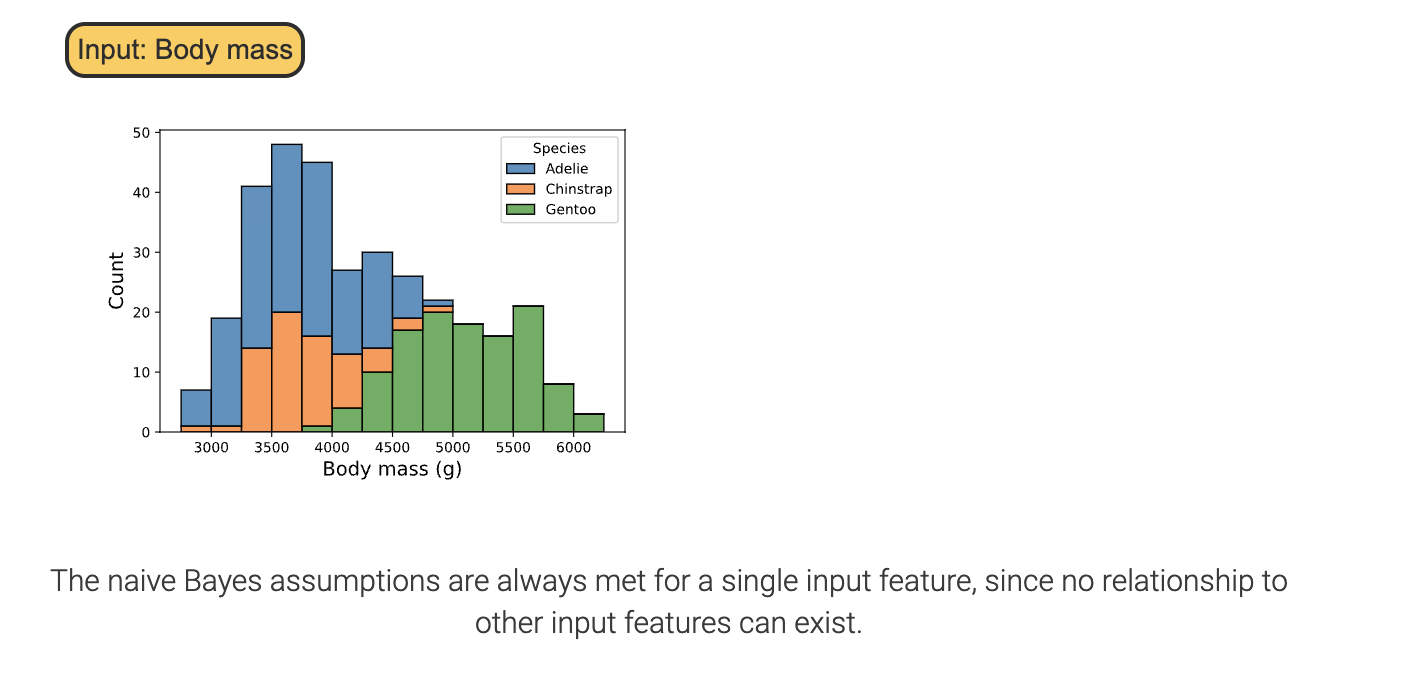
\includegraphics[width=0.8\textwidth]{imgs/nb_16.png}
	\end{figure}
\end{frame}

\begin{frame}{Naive Bayes Assumptions}
	\begin{figure}[ht]
		\centering
		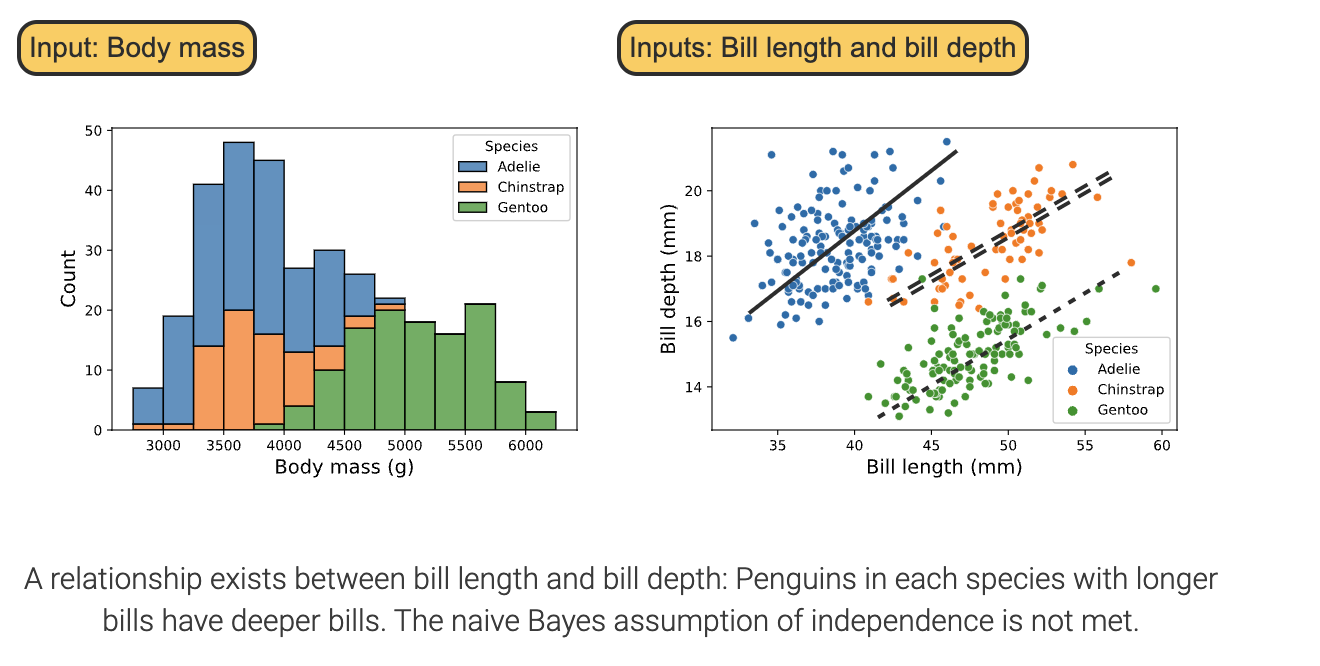
\includegraphics[width=0.8\textwidth]{imgs/nb_17.png}
	\end{figure}
\end{frame}

\begin{frame}{Practice Problem: Evaluating the naive Bayes assumptions.}
	\begin{figure}[ht]
		\centering
		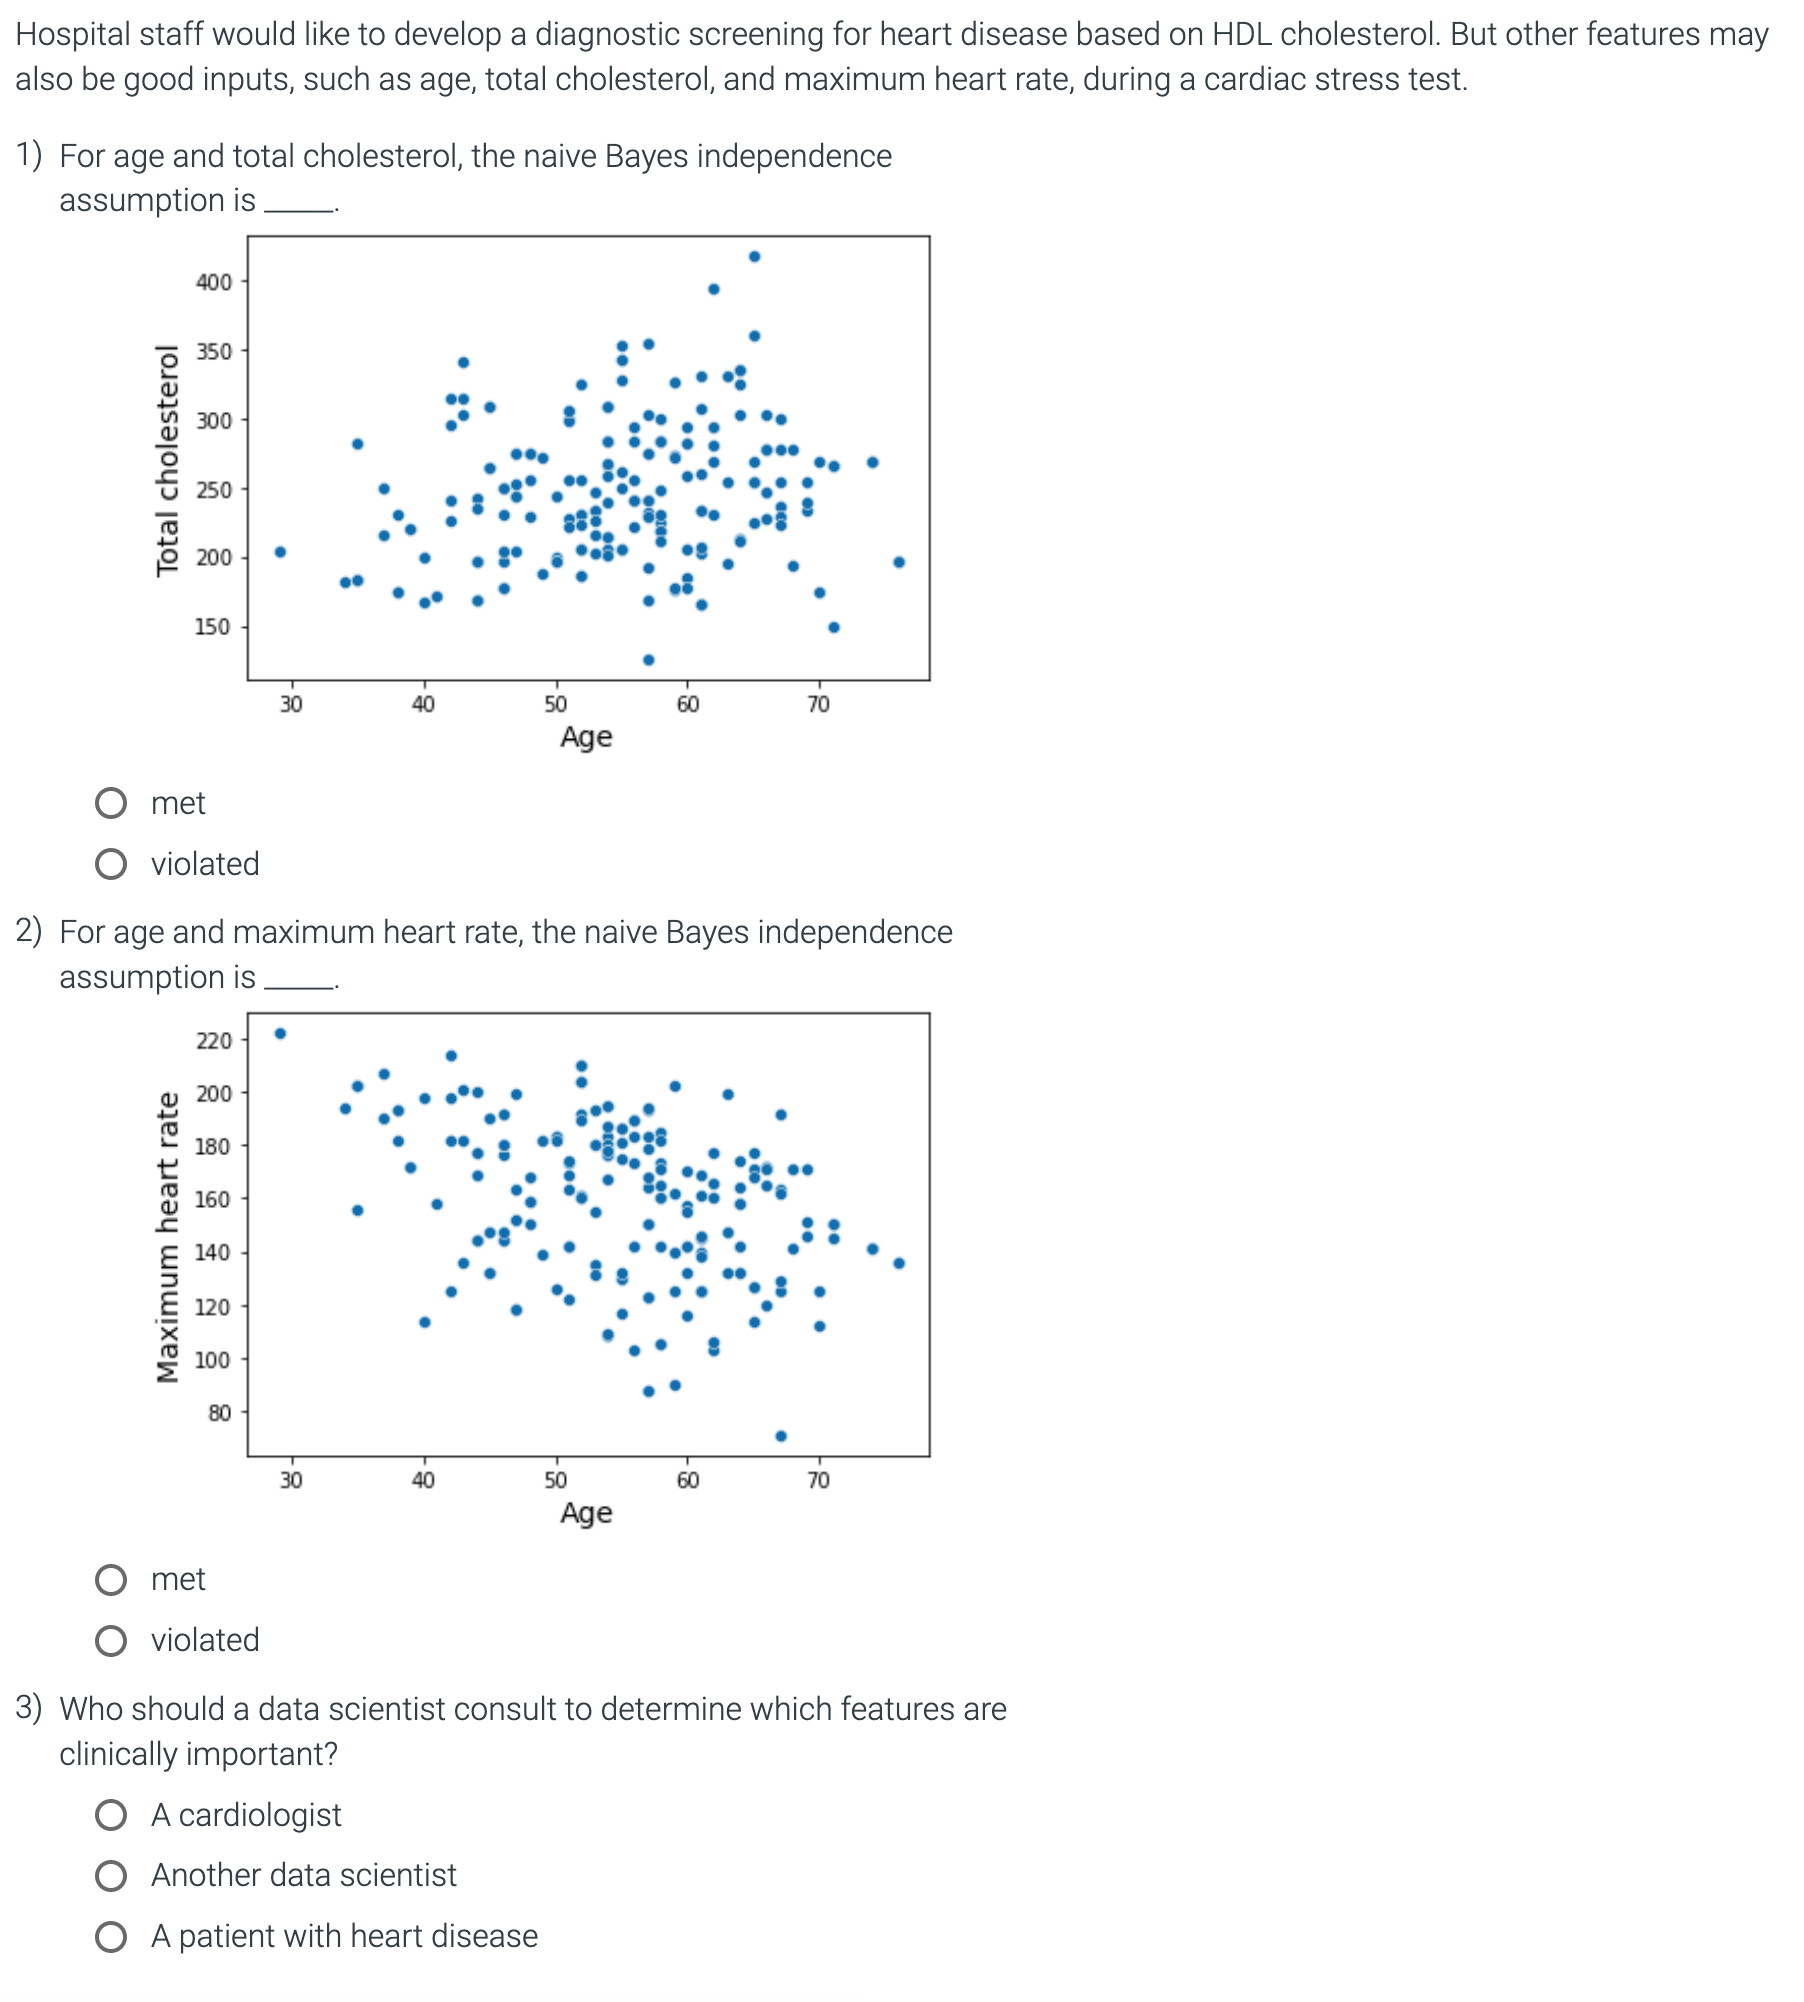
\includegraphics[width=0.6\textwidth]{imgs/nb_18.png}
	\end{figure}
\end{frame}

\begin{frame}{Practice Problem: Evaluating the naive Bayes assumptions.}
	\begin{figure}[ht]
		\centering
		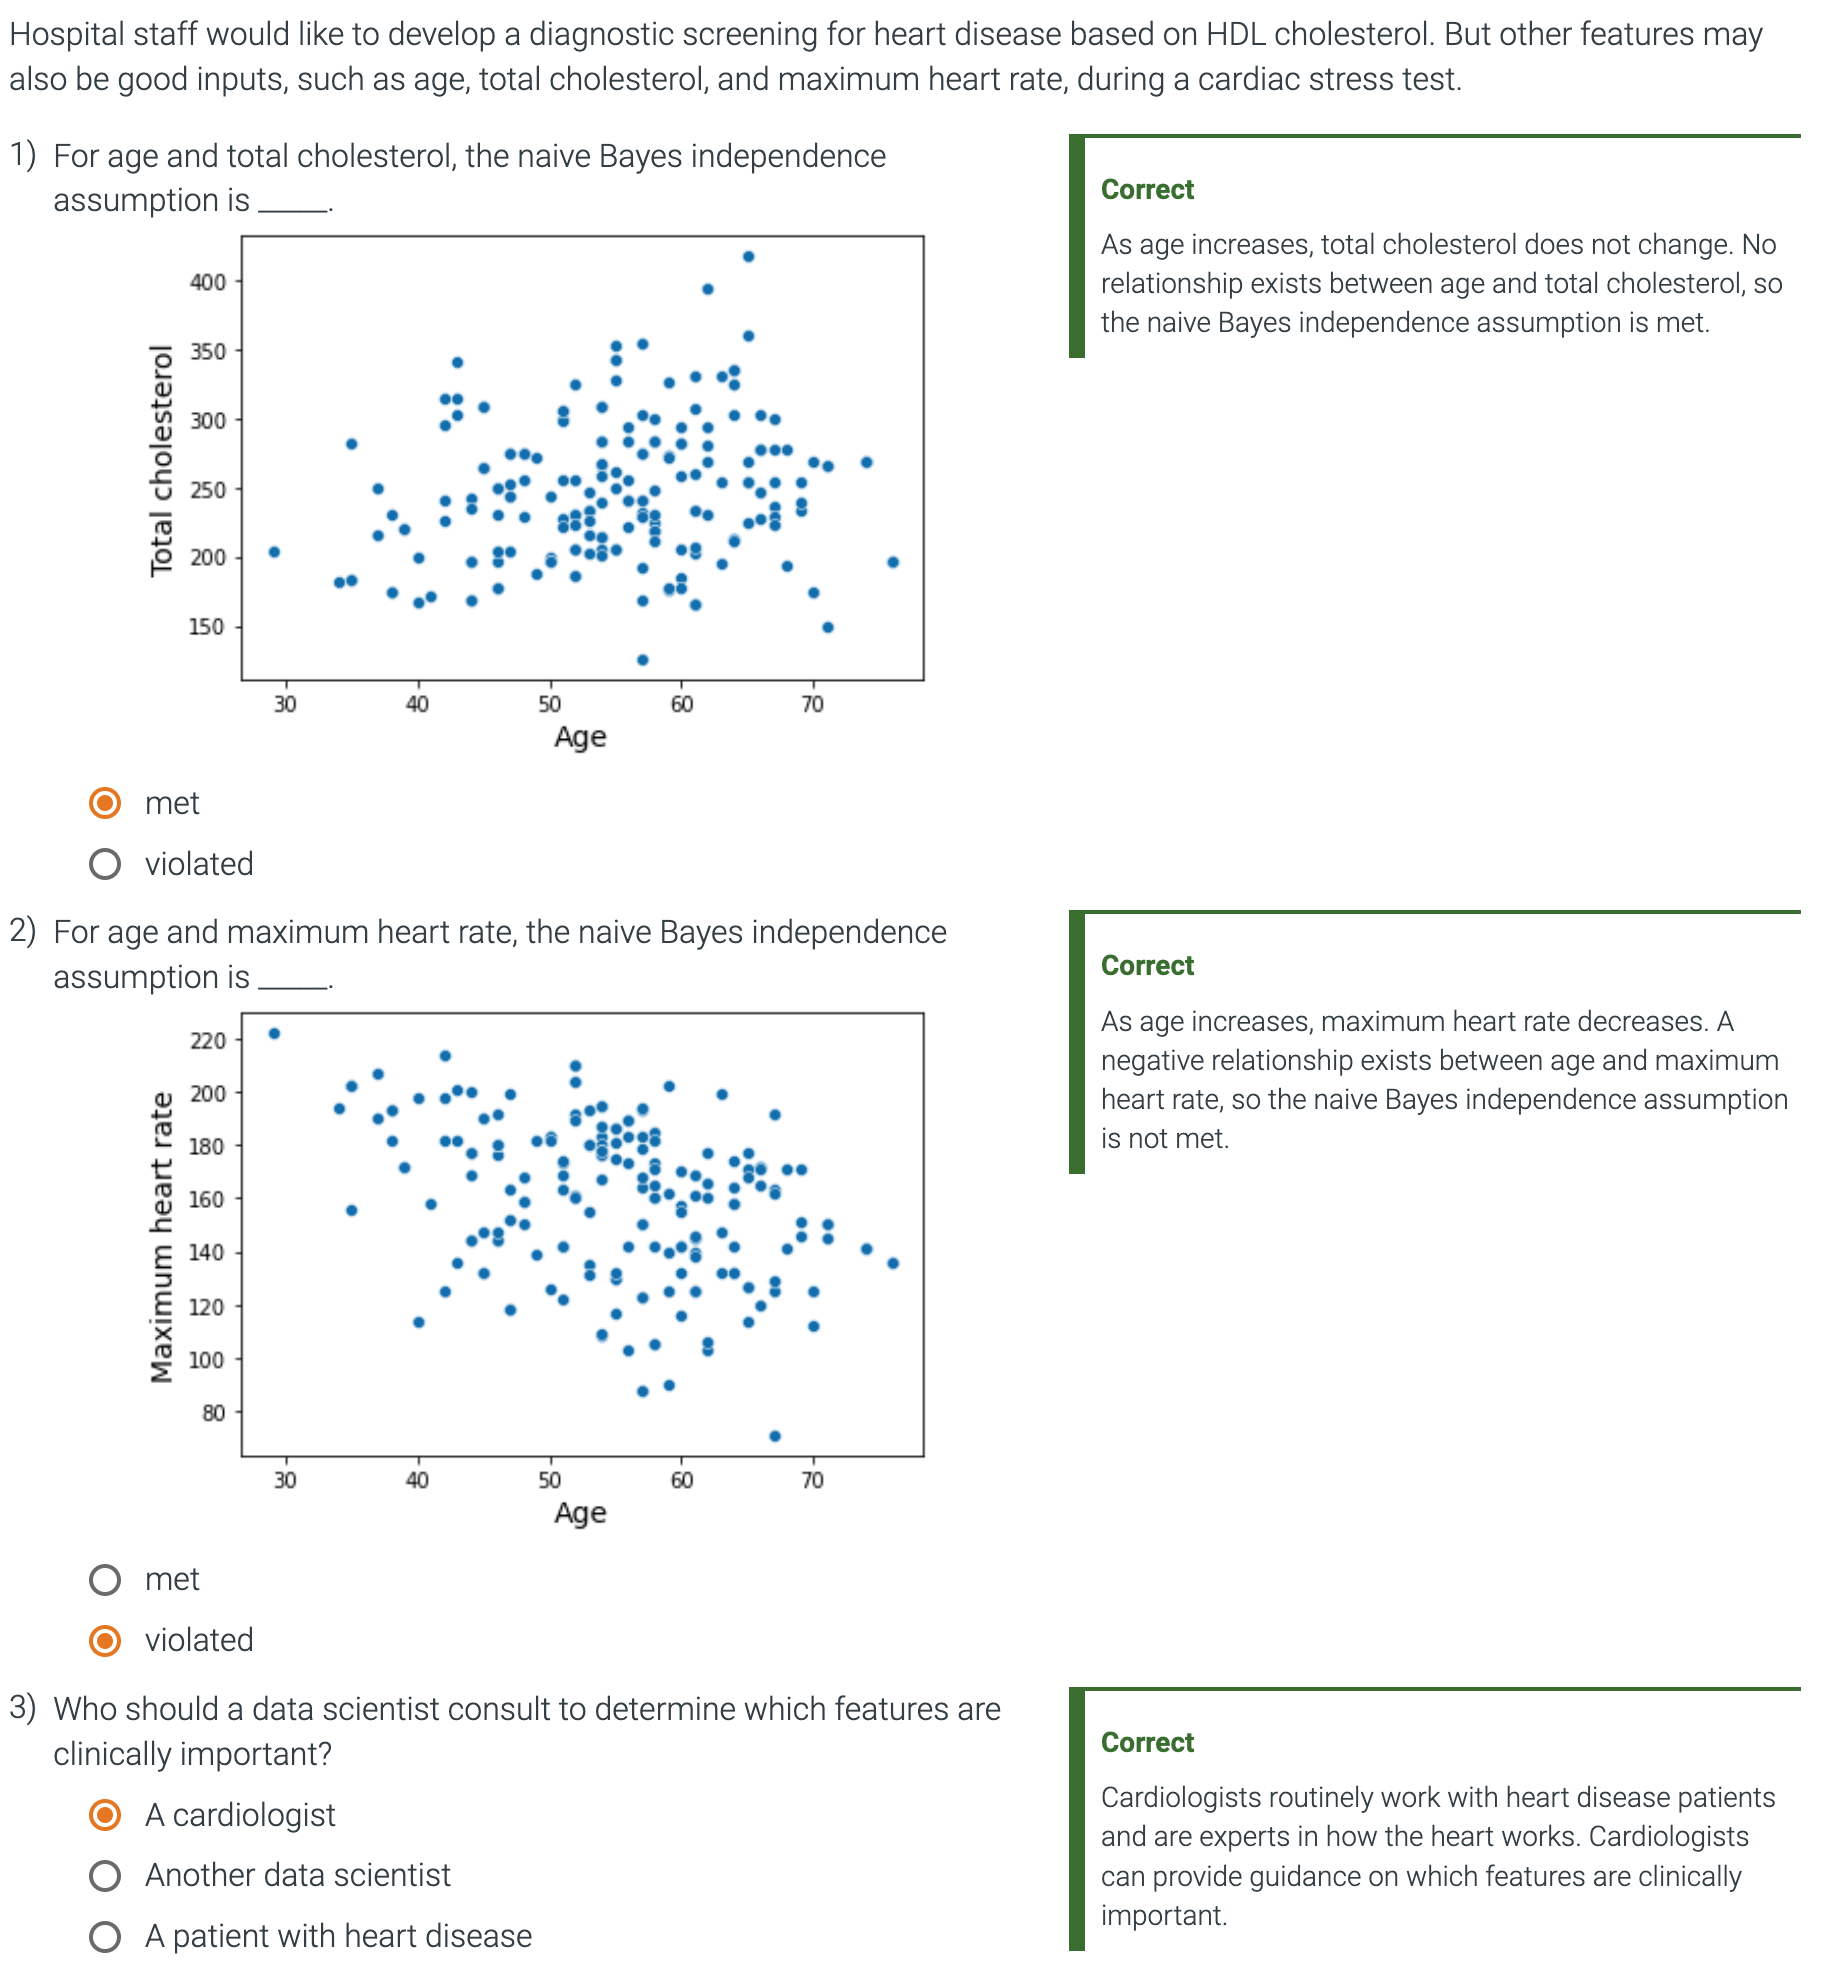
\includegraphics[width=0.6\textwidth]{imgs/nb_19.png}
	\end{figure}
\end{frame}

\section{Gaussian naive Bayes}
\begin{frame}{Gaussian naive Bayes}
	For categorical or discrete input features, sample probabilities can be calculated for each individual value of \(x\). For numerical input features,
	continuous probability distributions are used instead of sample probabilities. A \textbf{continuous probability distribution} is a mathematical
	function that describes the probability that a certain value of a random variable occurs.
	
	The most common choice for numerical input features is the Gaussian, or normal, distribution. The \textbf{normal distribution}, denoted
	normal \((\mu, \sigma)\), is a symmetric, bell-shaped distribution with two parameters: the mean, \(\mu\), and the standard deviation \(\sigma\). The normal
	distribution provides a good approximation for many input features.
	$$
	f(x)=\frac{1}{\sqrt{2 \pi \sigma^{2}}} \exp \left((x-\mu)^{2} / 2 \sigma^{2}\right)
	$$
\end{frame}

\begin{frame}{Gaussian naive Bayes}
\textbf{Gaussian naive Bayes} uses the normal distribution as an approximation to the conditional probability \(P\left(x \mid y_{i}\right)\). One normal distribution is fitted to each class and used to calculate the posterior probabilities.
\end{frame}

\begin{frame}{Approximating Conditional Probabilities with the Normal Distribution}
		\begin{figure}[ht]
		\centering
		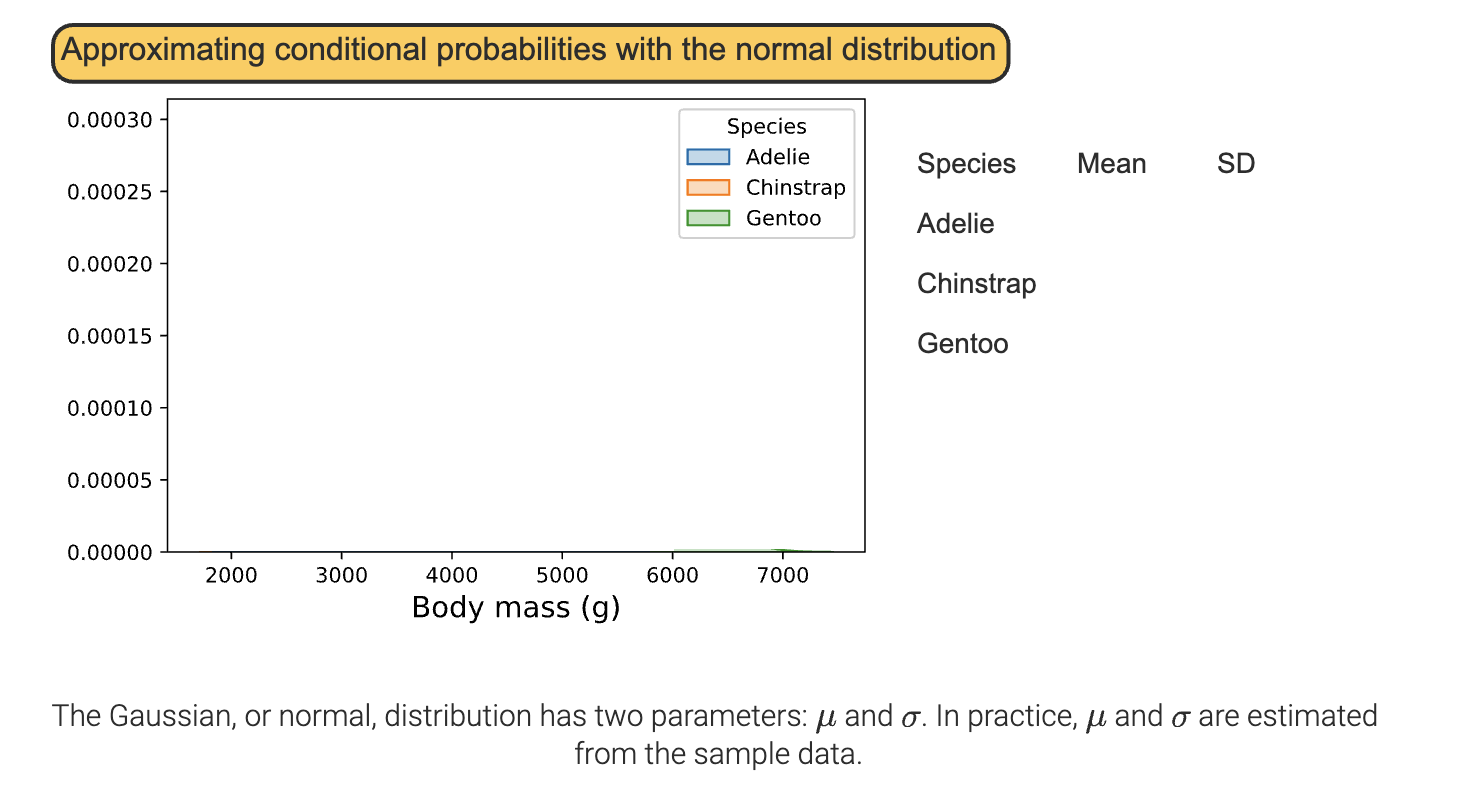
\includegraphics[width=0.8\textwidth]{imgs/nb_20.png}
	\end{figure}
\end{frame}

\begin{frame}{Approximating Conditional Probabilities with the Normal Distribution}
	\begin{figure}[ht]
		\centering
		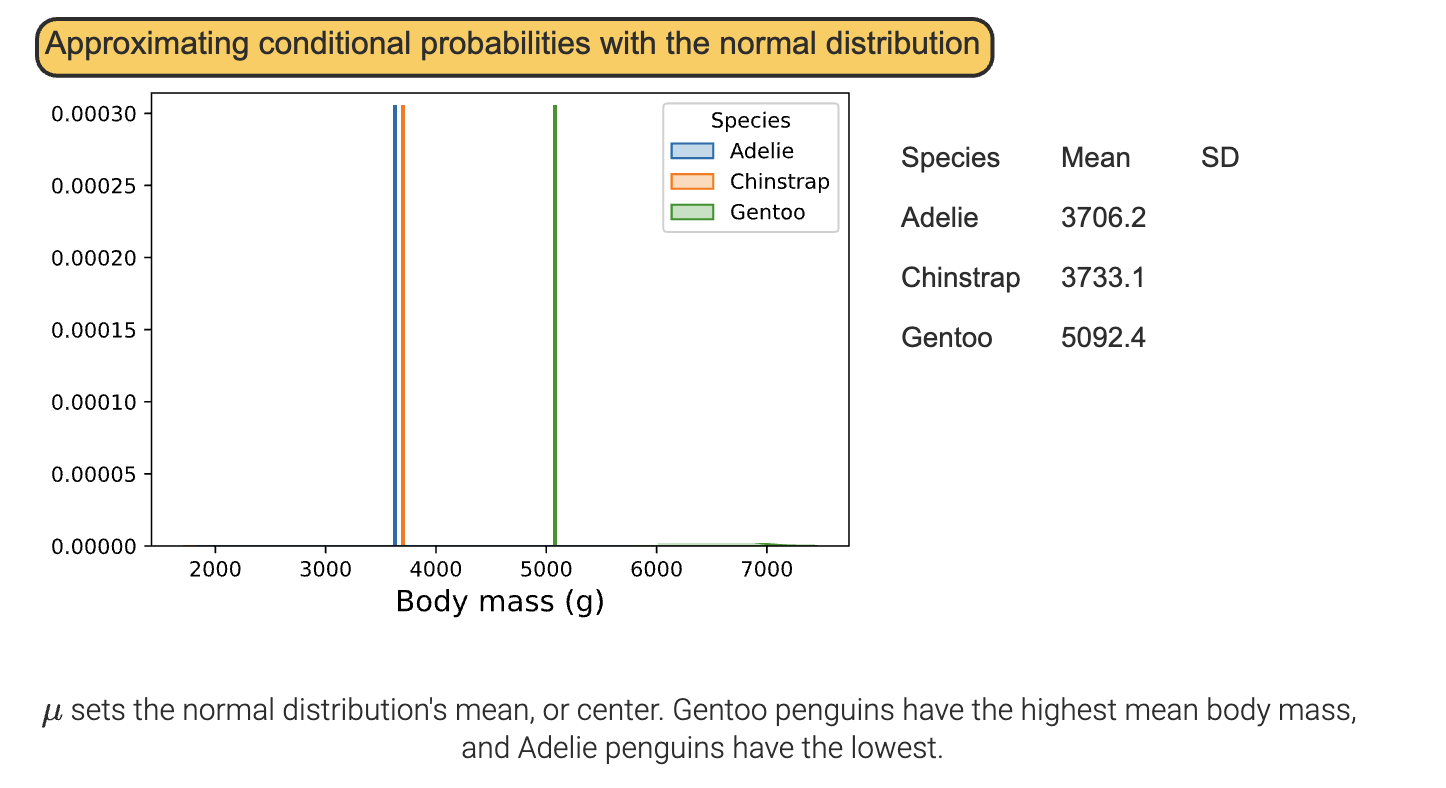
\includegraphics[width=0.8\textwidth]{imgs/nb_21.png}
	\end{figure}
\end{frame}

\begin{frame}{Approximating Conditional Probabilities with the Normal Distribution}
	\begin{figure}[ht]
		\centering
		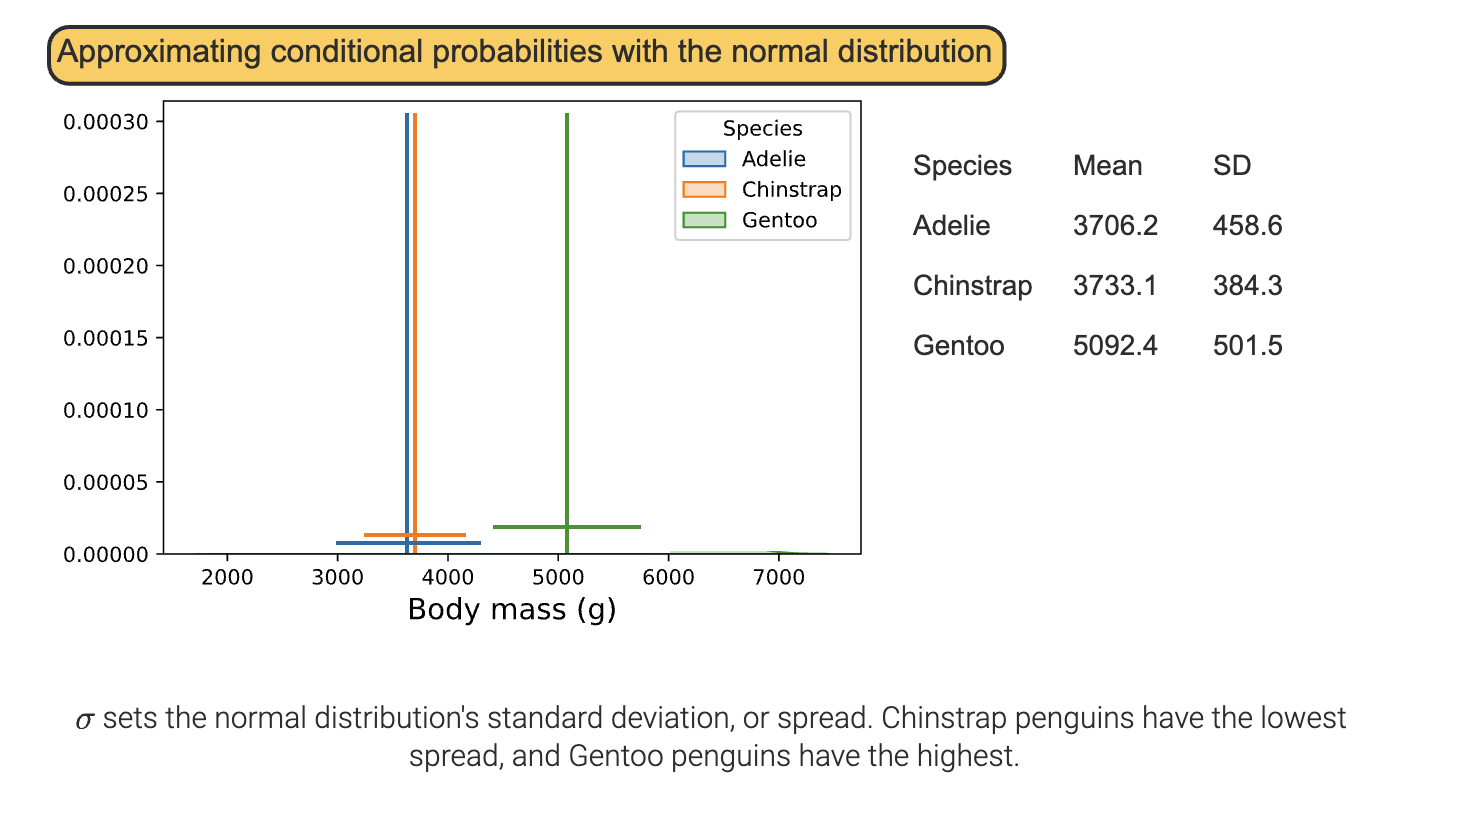
\includegraphics[width=0.8\textwidth]{imgs/nb_22.png}
	\end{figure}
\end{frame}

\begin{frame}{Approximating Conditional Probabilities with the Normal Distribution}
	\begin{figure}[ht]
		\centering
		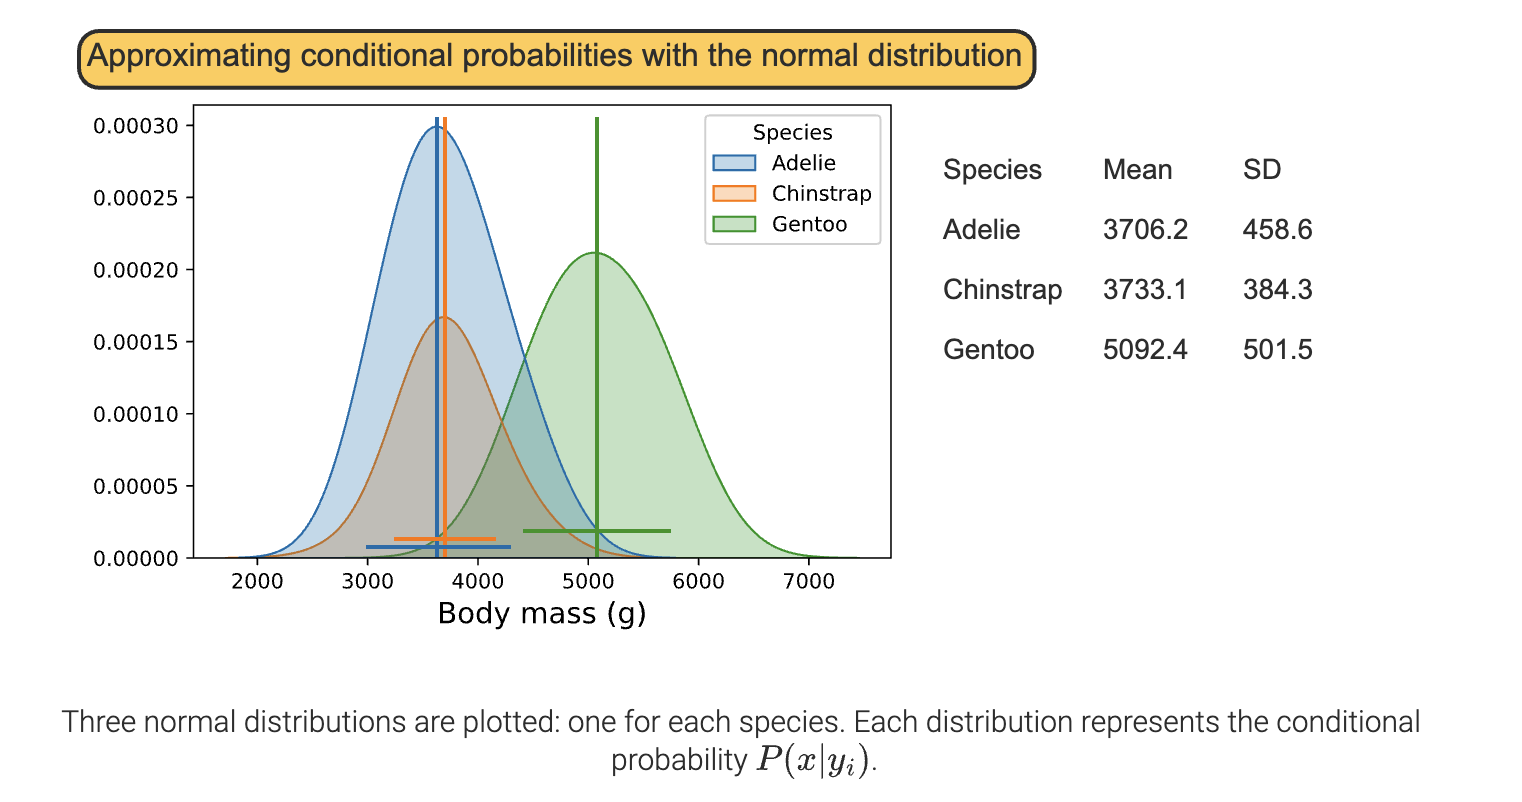
\includegraphics[width=0.8\textwidth]{imgs/nb_23.png}
	\end{figure}
\end{frame}

\begin{frame}{Practice Problem: Normal approximation for heart disease screening.}
		\begin{figure}[ht]
		\centering
		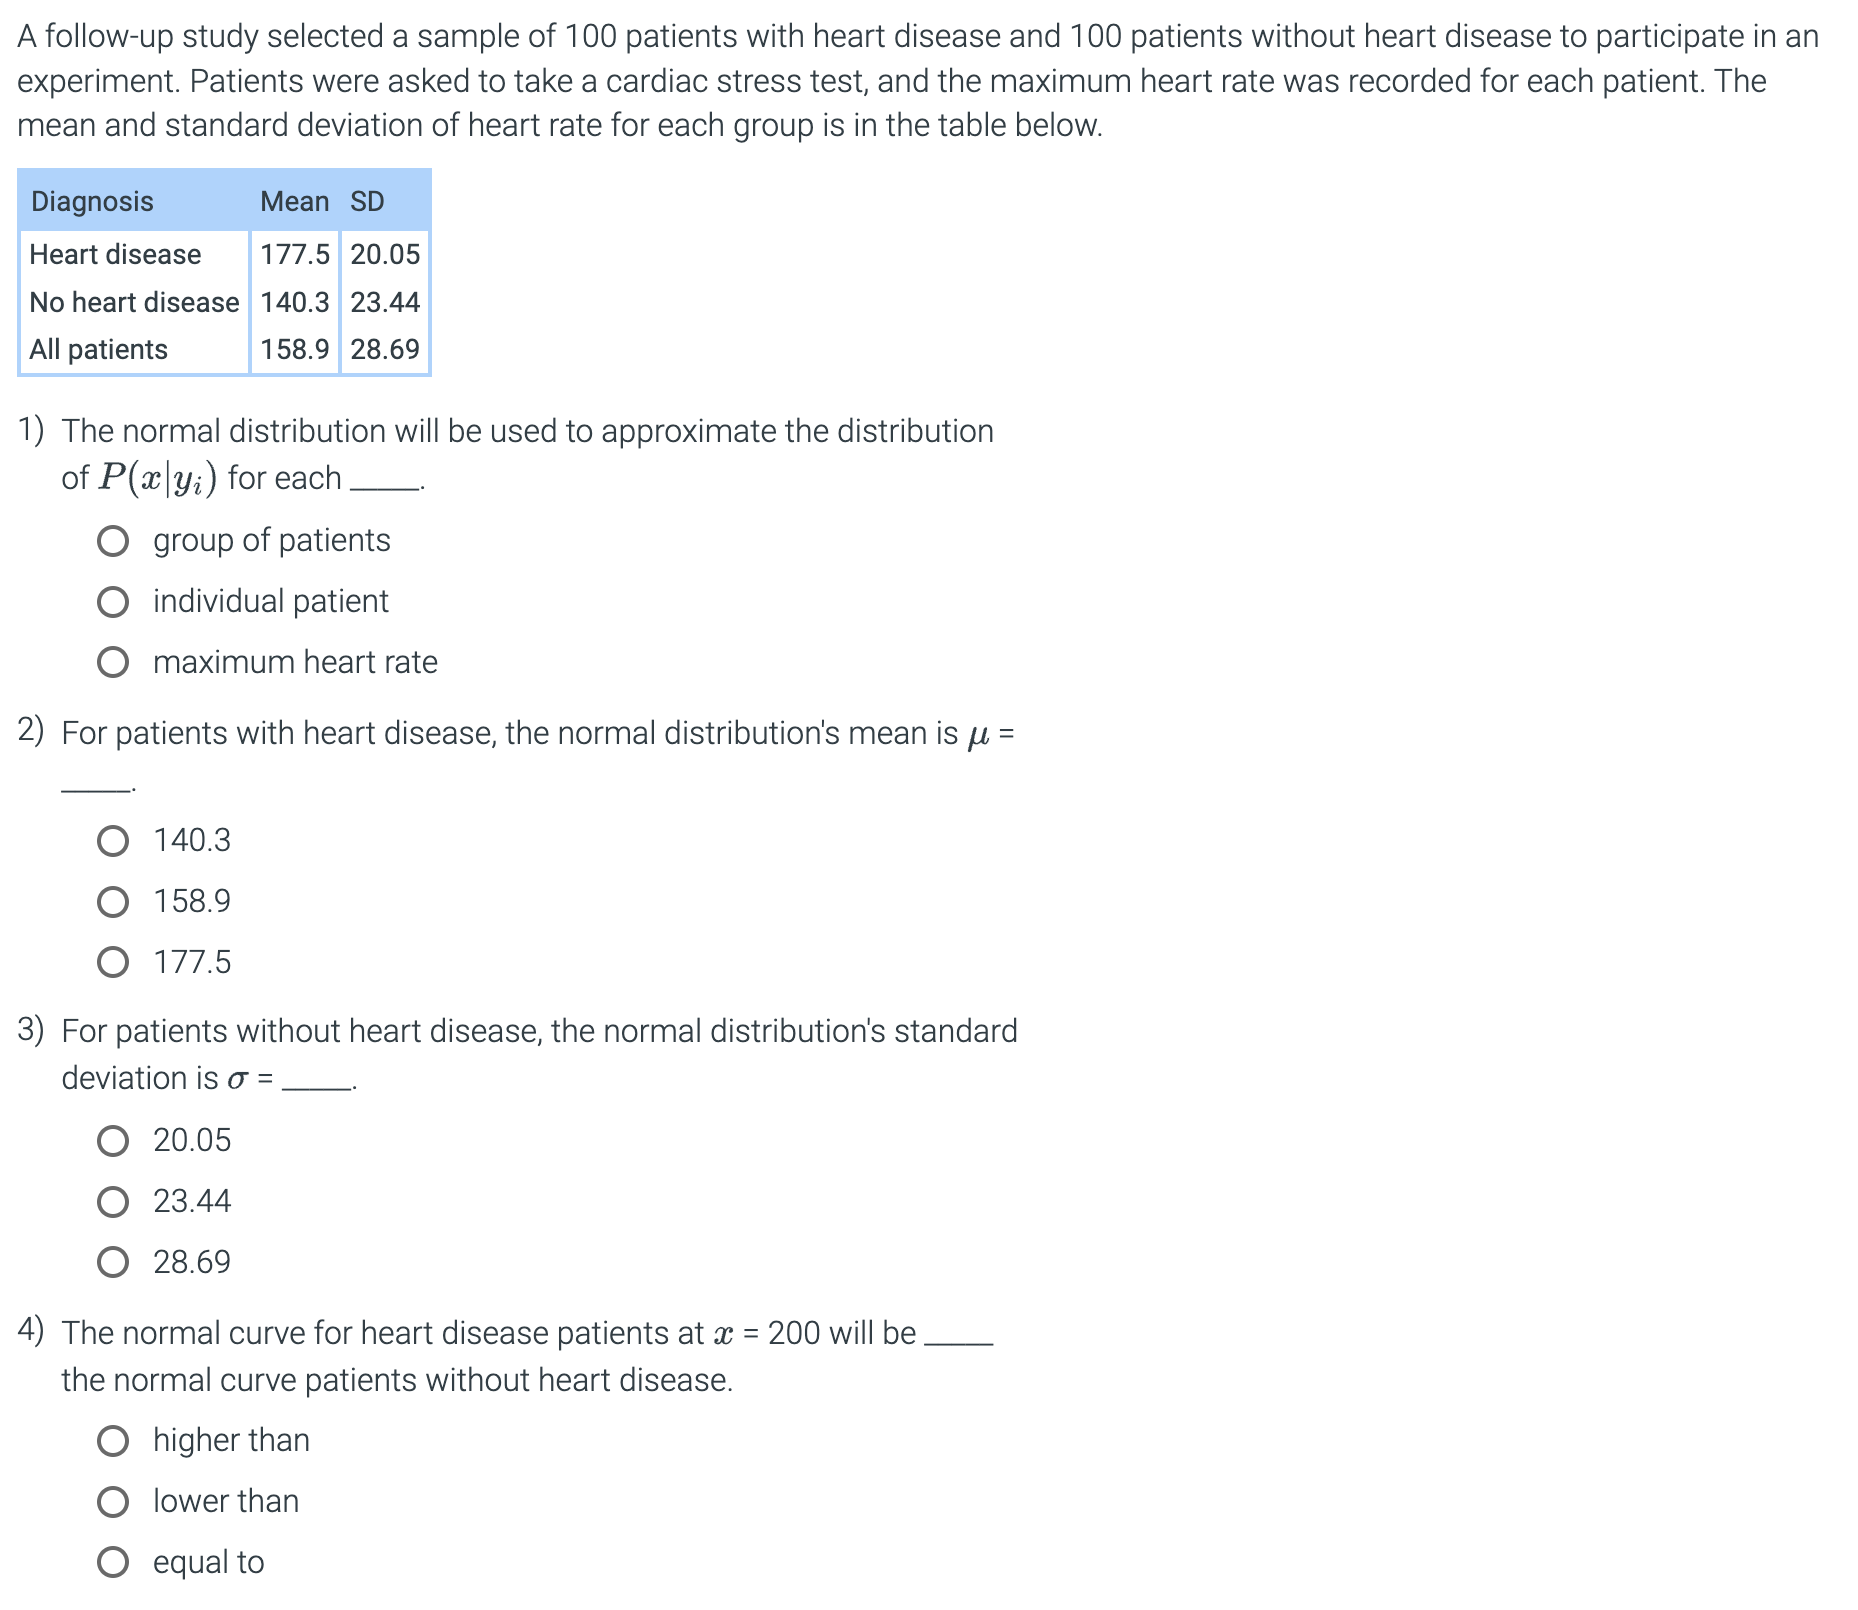
\includegraphics[width=0.6\textwidth]{imgs/nb_24.png}
	\end{figure}
\end{frame}

\begin{frame}{Practice Problem: Normal approximation for heart disease screening.}
	\begin{figure}[ht]
		\centering
		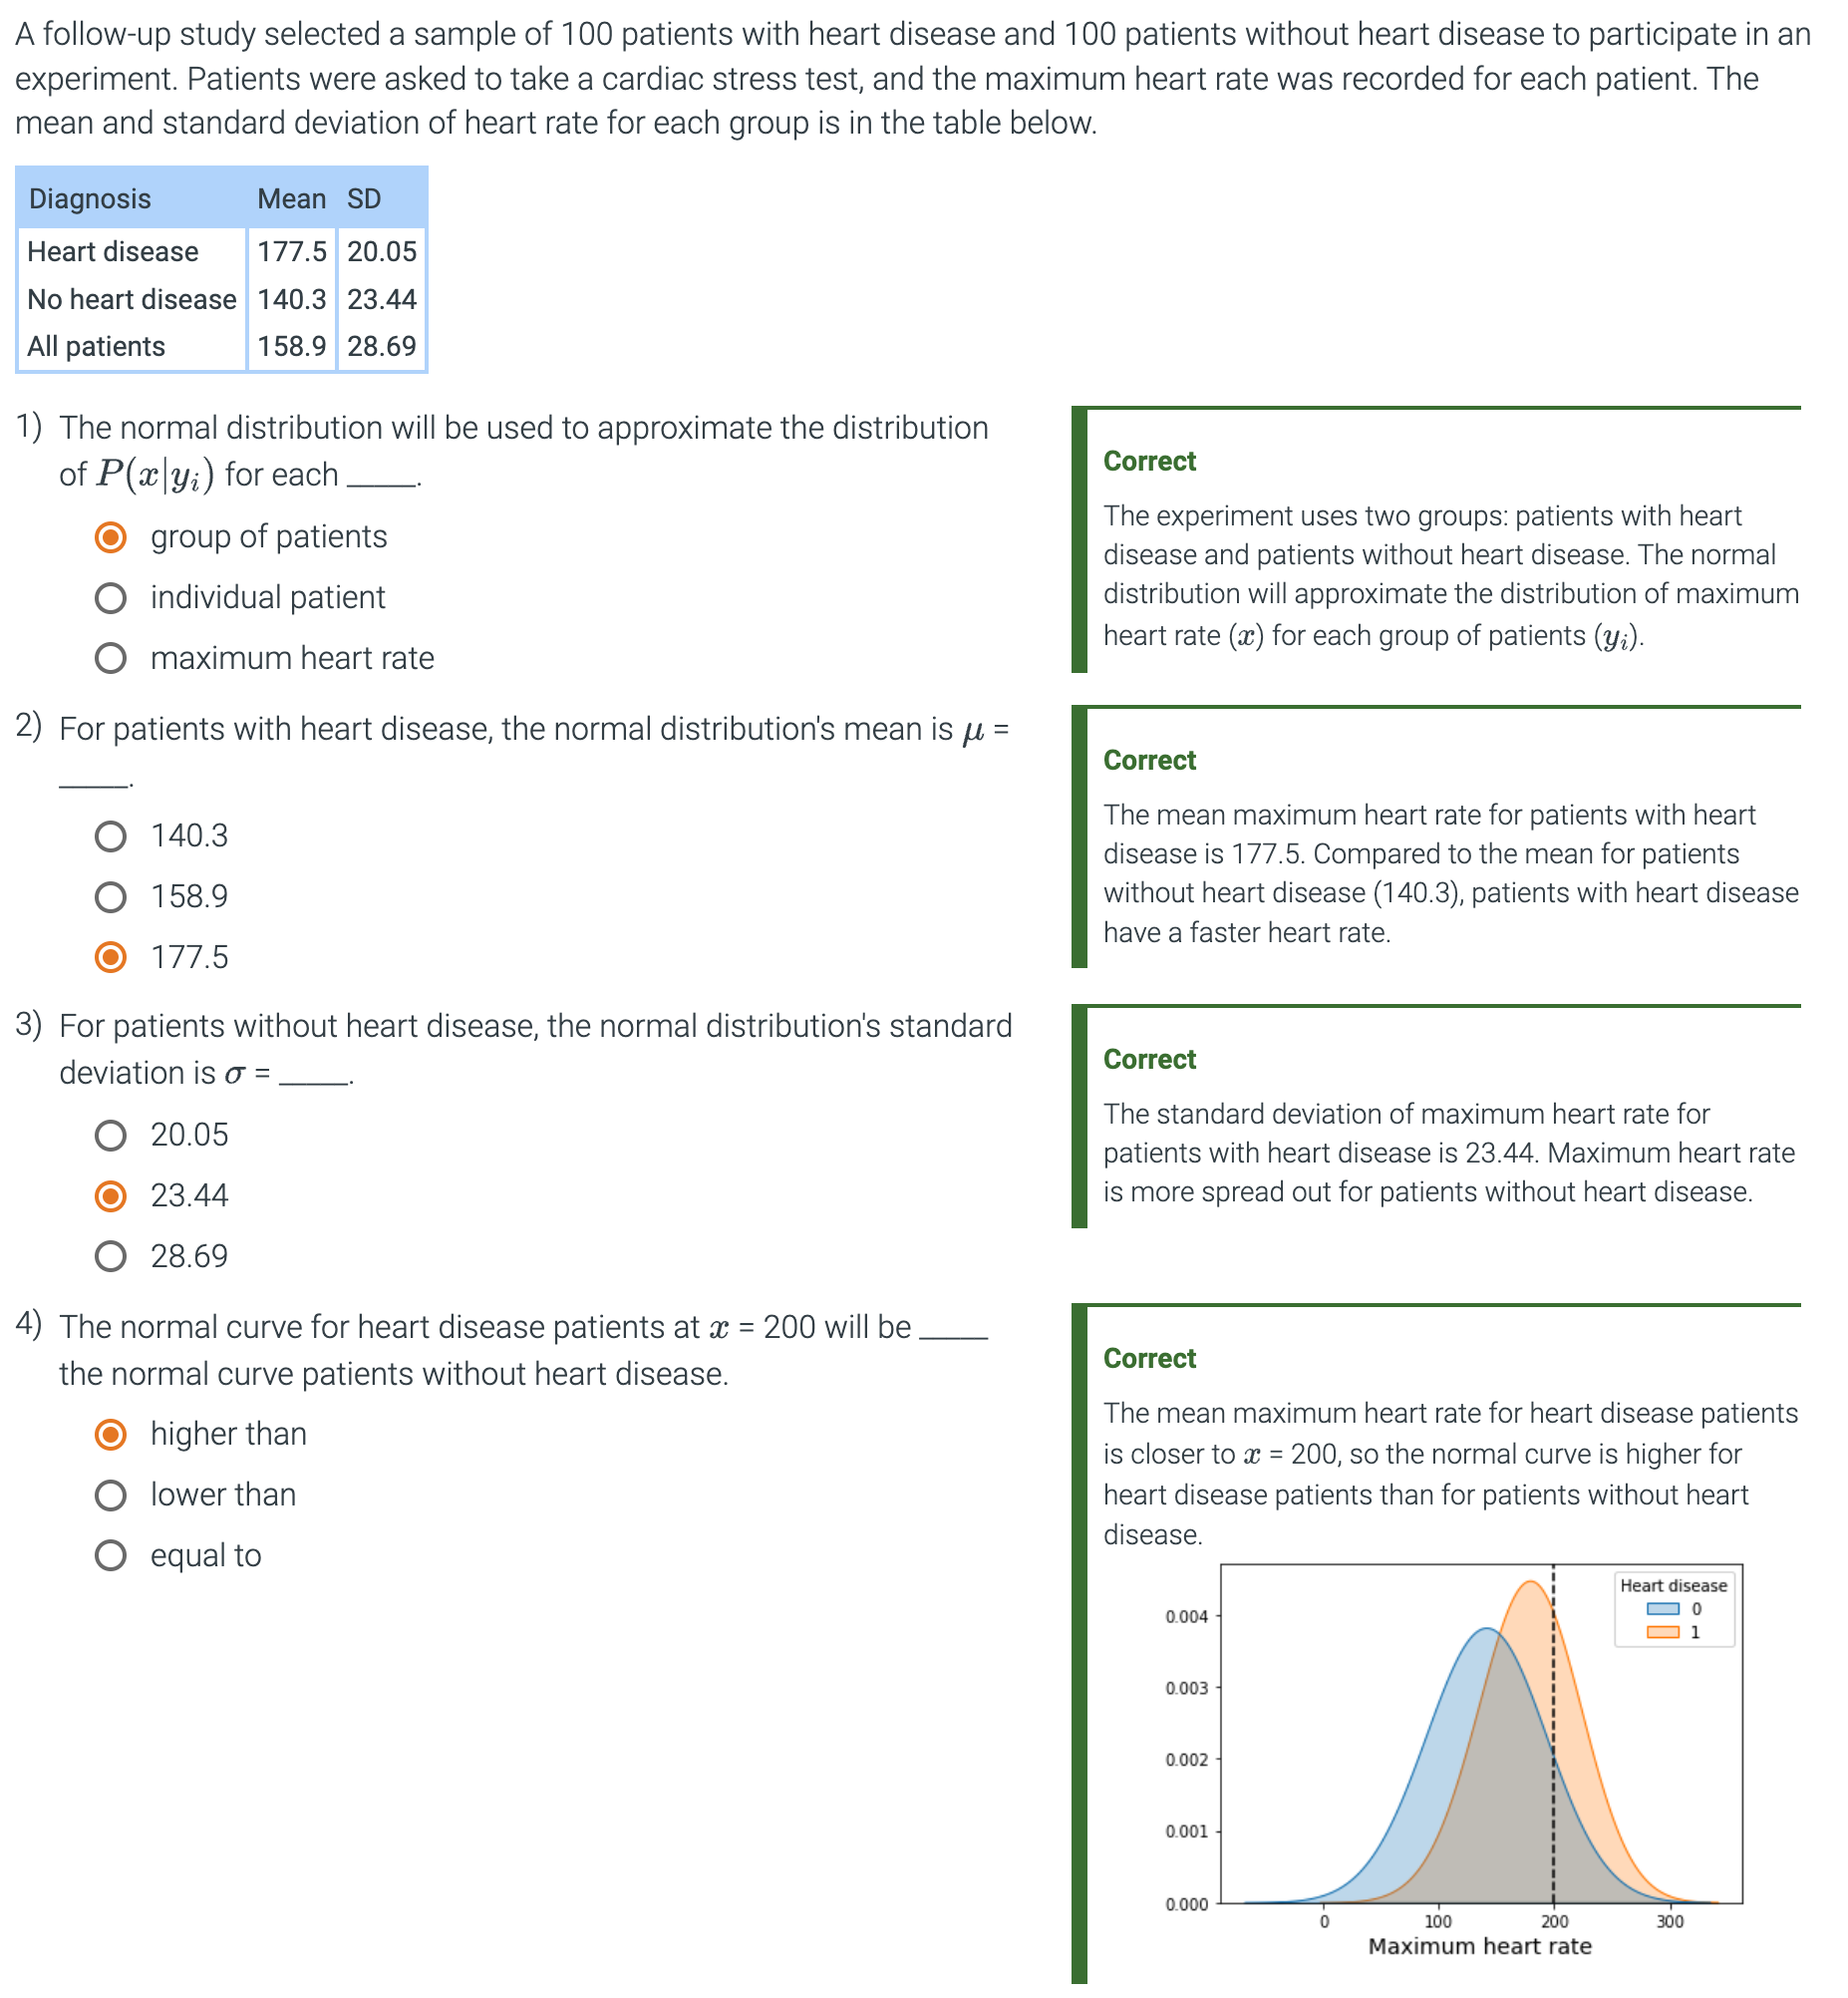
\includegraphics[width=0.6\textwidth]{imgs/nb_25.png}
	\end{figure}
\end{frame}

\section{Bayesian Priors}
\begin{frame}{Bayesian Priorsi}
	\textbf{Bayesian models}, including naive Bayes classifiers, incorporate prior assumptions about the probability a given event occurs in the model's
	predictions. 
	\begin{itemize}
		\item  Ex: By default, most implementations of naive Bayes classification use the sample probabilities of each class, \(P\left(y_{i}\right)\), as the
		prior probabilities.
		\item  But the prior probabilities may be adjusted based on outside information. Adjusting the prior probabilities may have an impact on the model's predictions and performance.
	\end{itemize}
\end{frame}

\begin{frame}{Effect of prior probabilities on predictions.}
		\begin{figure}[ht]
		\centering
		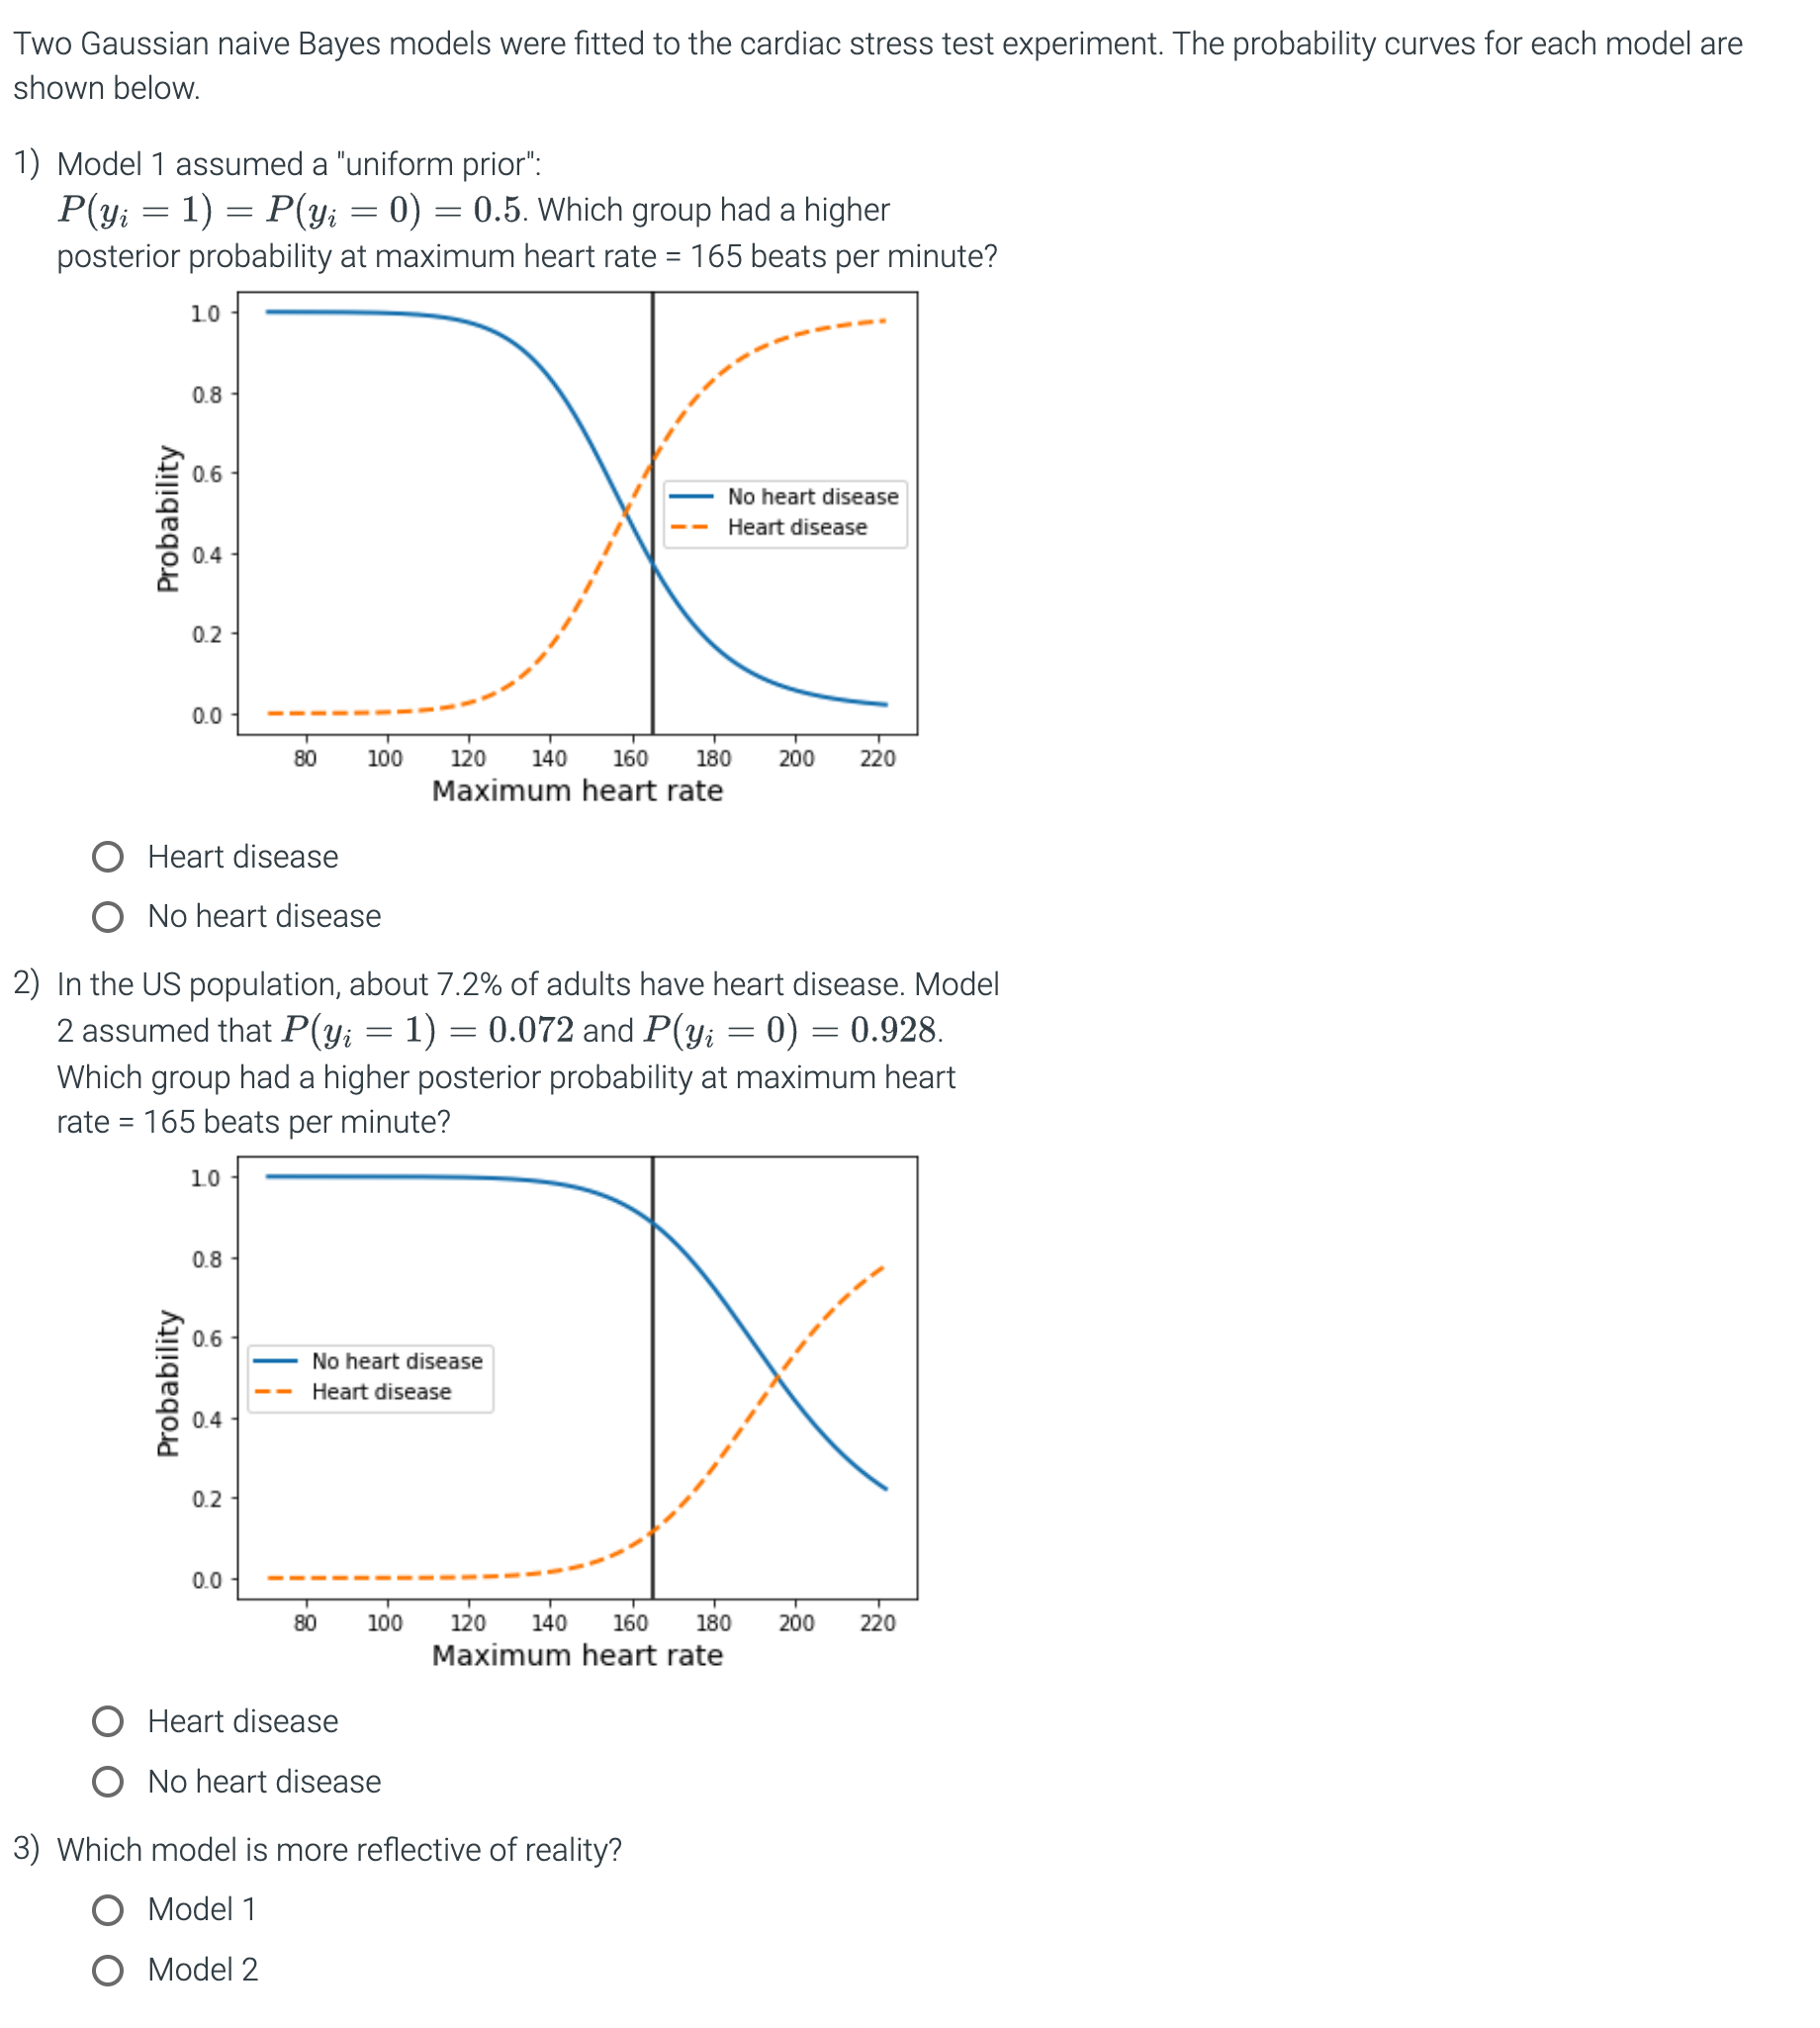
\includegraphics[width=0.6\textwidth]{imgs/nb_26.png}
	\end{figure}
\end{frame}

\begin{frame}{Effect of prior probabilities on predictions.}
	\begin{figure}[ht]
		\centering
		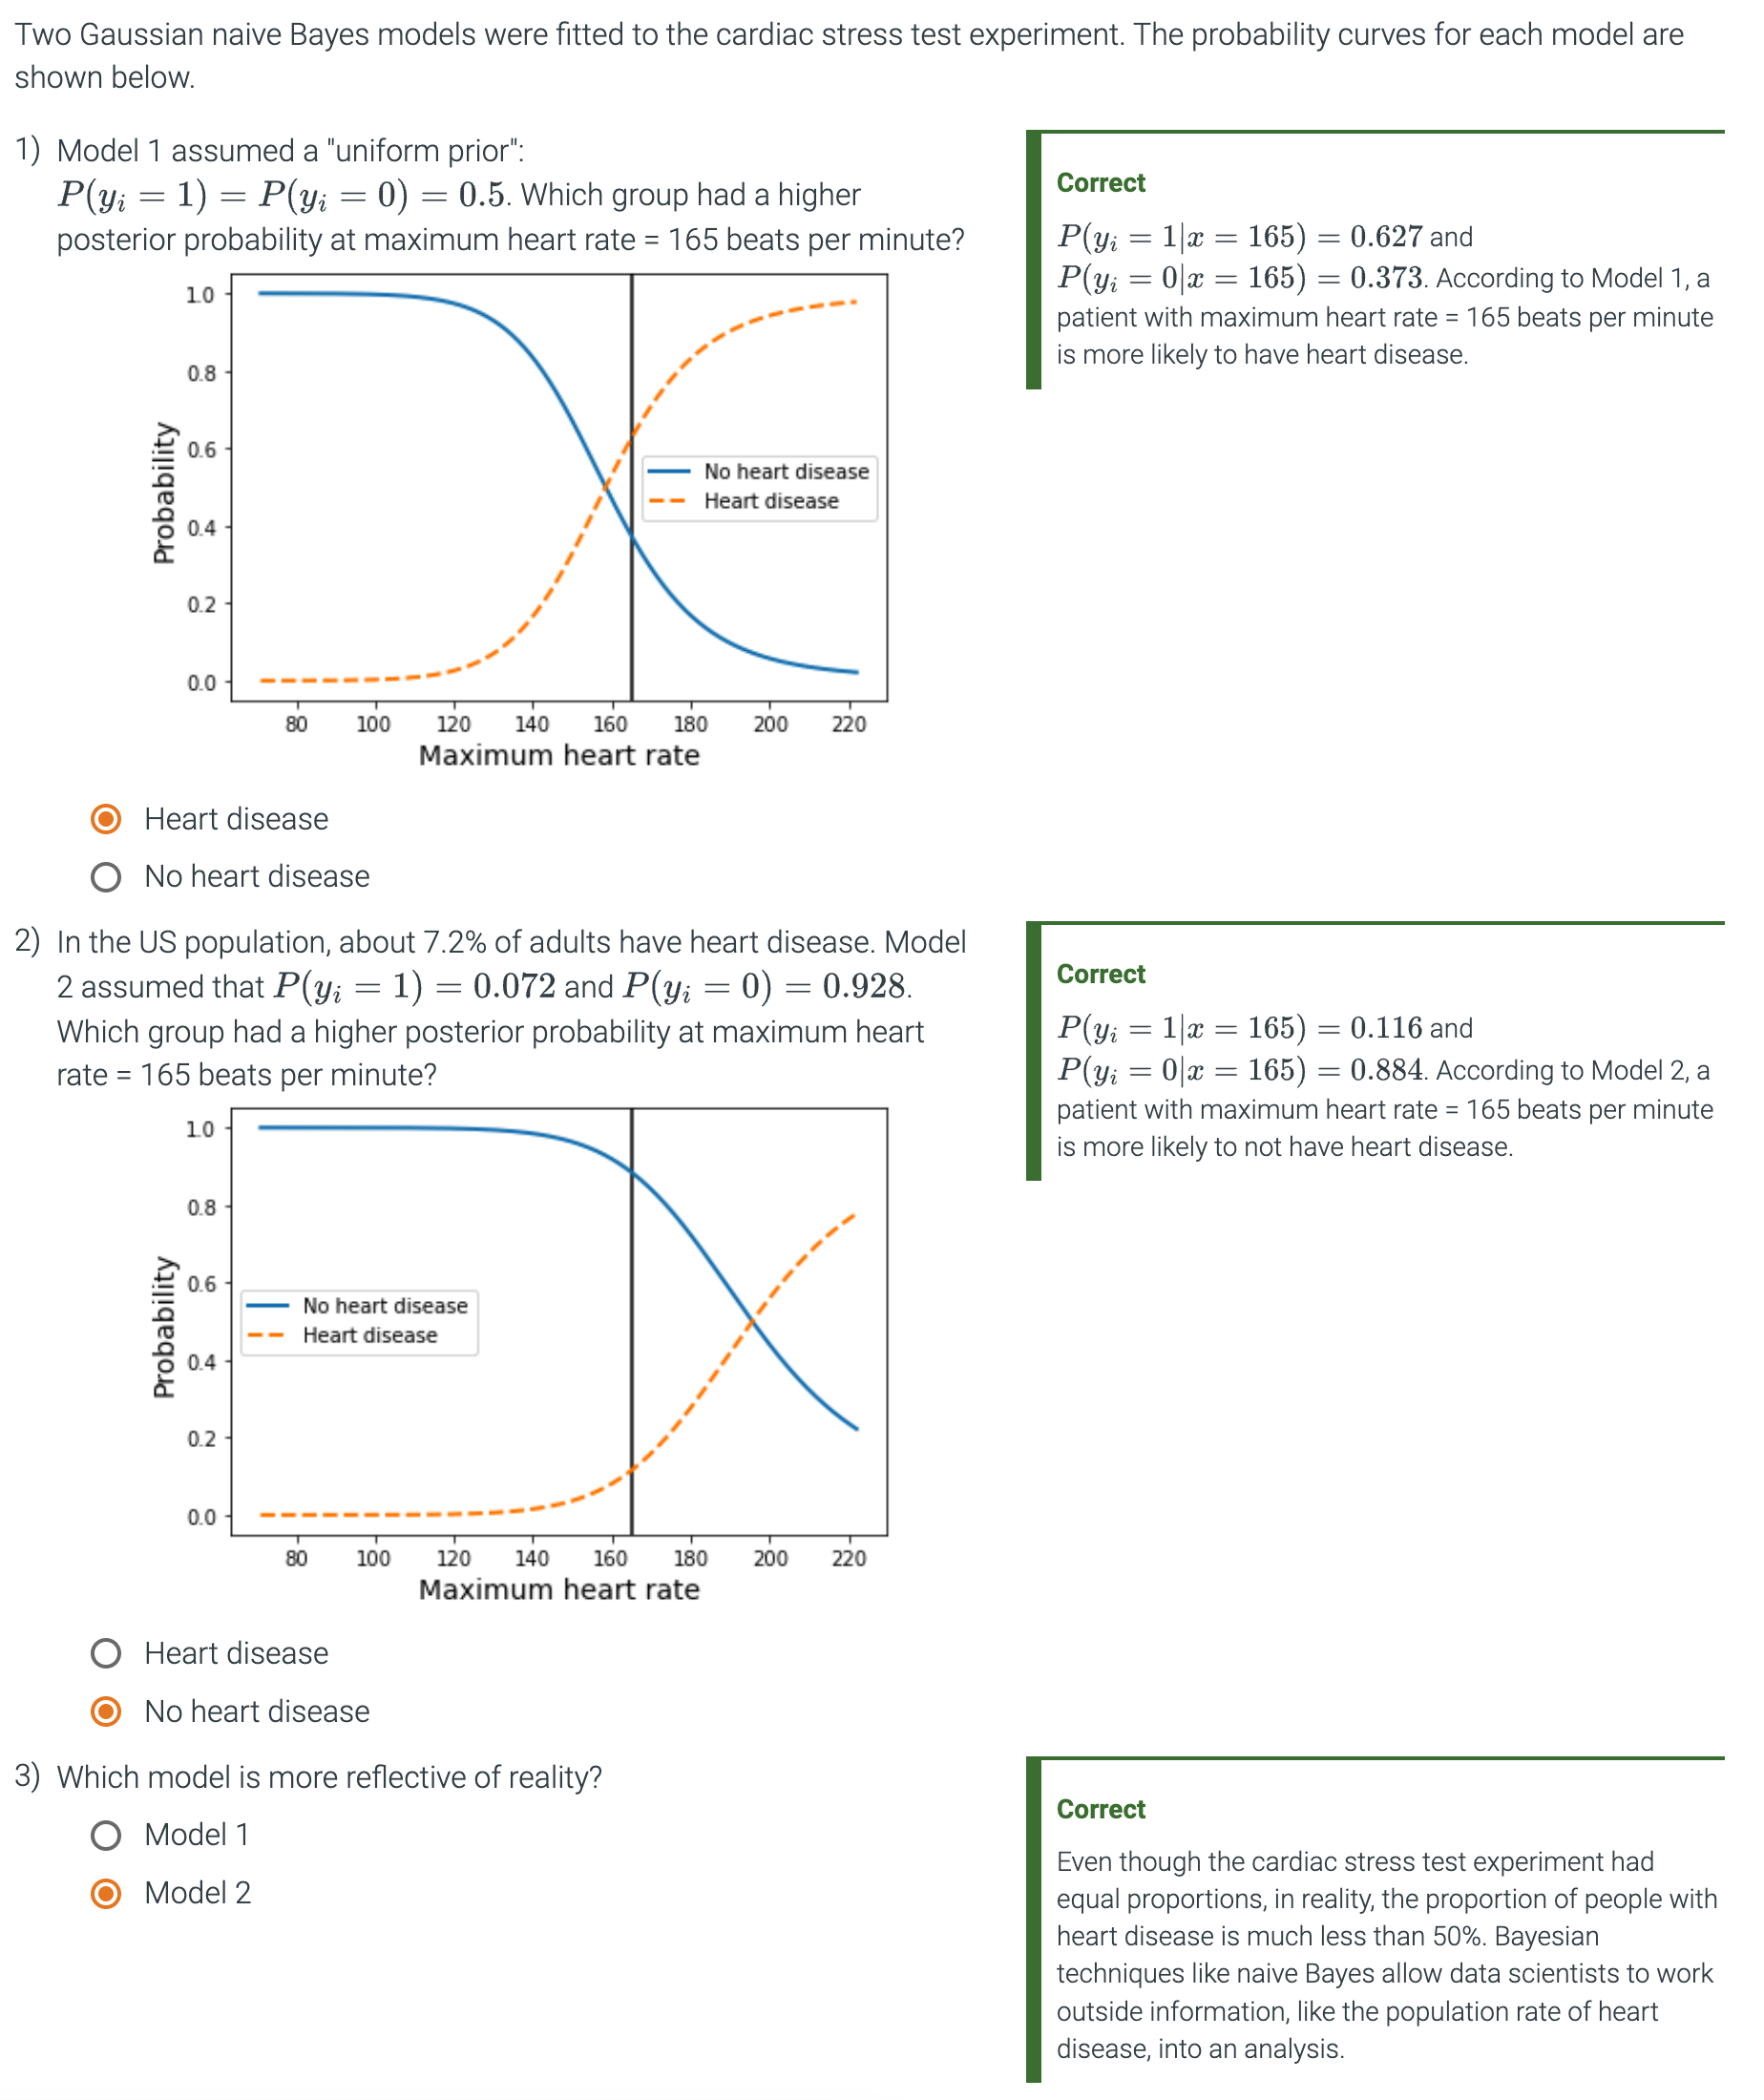
\includegraphics[width=0.6\textwidth]{imgs/nb_27.png}
	\end{figure}
\end{frame}

\section{Advantages and Disadvantages}
\begin{frame}{Advantages and disadvantages}
	Naive Bayes' predictions are fast to compute, since predictions are based on conditional probabilities. 
	\begin{itemize}
		\item For large datasets that require fast predictions, the computational advantages make naive Bayes a good choice. But the naive Bayes assumptions are often unrealistic.
		\item A tradeoff exists between computational ease and theoretical requirements. If the predictions are fast and accurate, naive Bayes may still be useful despite violated assumptions.
	\end{itemize}
\end{frame}

\begin{frame}{Naive Bayes Assumptions.}
		\begin{figure}[ht]
		\centering
		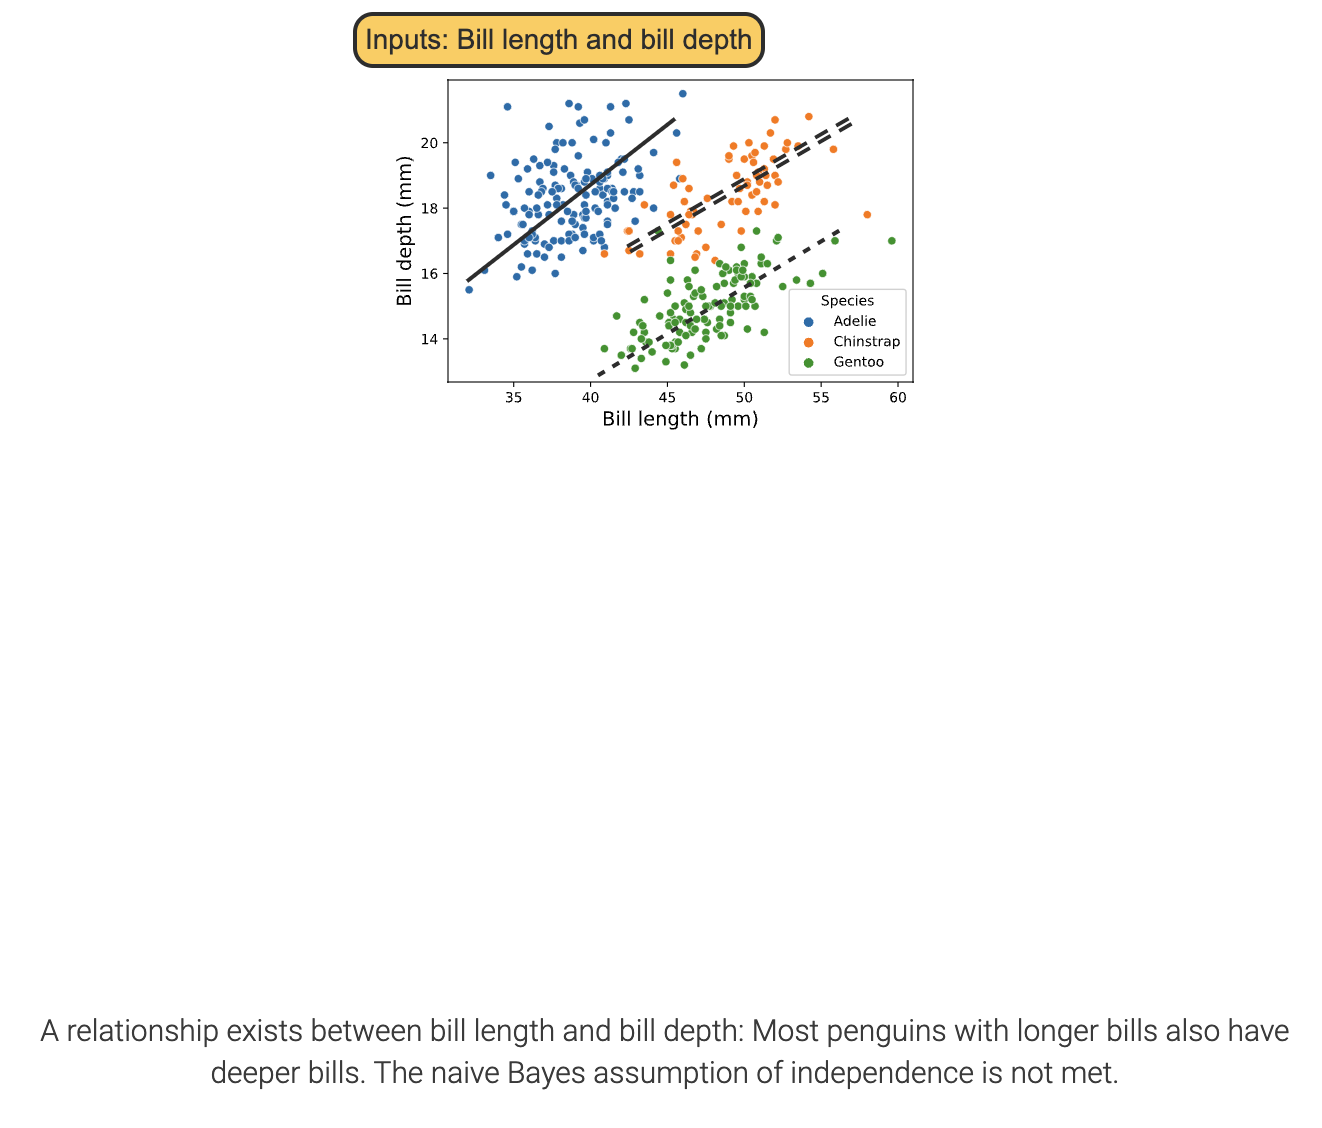
\includegraphics[width=0.8\textwidth]{imgs/nb_28.png}
	\end{figure}
\end{frame}

\begin{frame}{Naive Bayes Assumptions.}
	\begin{figure}[ht]
		\centering
		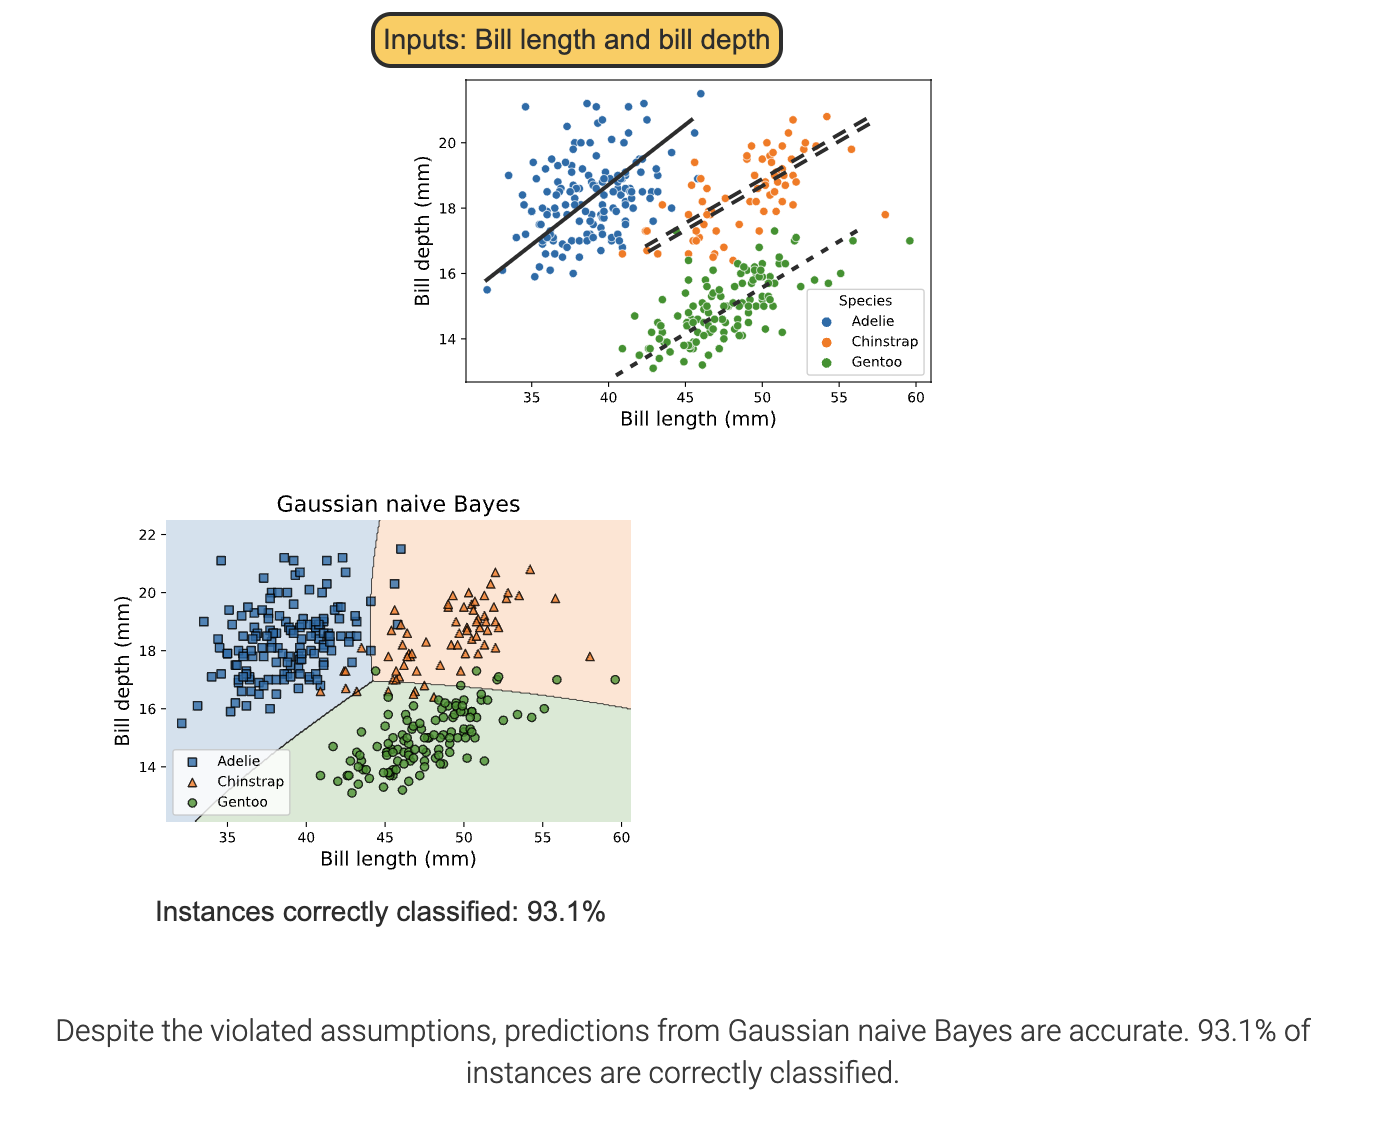
\includegraphics[width=0.8\textwidth]{imgs/nb_29.png}
	\end{figure}
\end{frame}

\begin{frame}{Naive Bayes Assumptions.}
	\begin{figure}[ht]
		\centering
		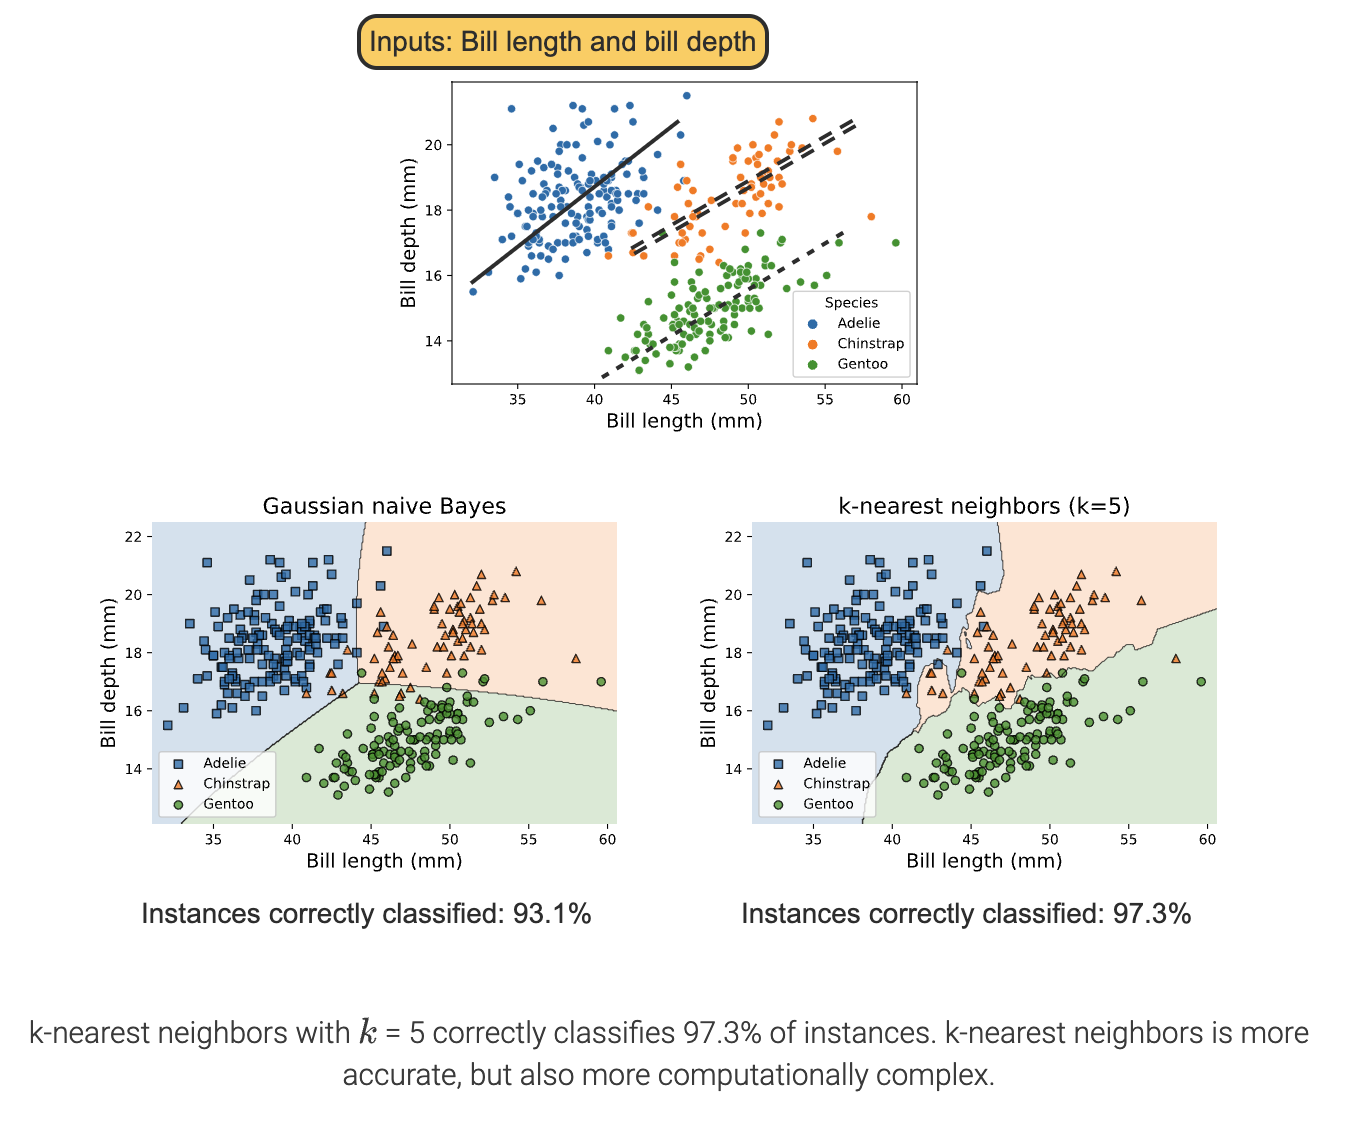
\includegraphics[width=0.8\textwidth]{imgs/nb_30.png}
	\end{figure}
\end{frame}
\end{document}


